\documentclass[11pt,a4paper,twoside,pdf]{article}

% Paquetes (añade otros si los necesitas):

\usepackage[T1]{fontenc}
\usepackage[utf8]{inputenc}


\usepackage[pdftex,final]{graphicx}
\bibliographystyle{unsrt} % We choose the "plain" reference style

% Style package
% Font Package (Palatino)
\usepackage{mathpazo}
% Packages for specific capabilities
\usepackage{rotating} % for text rotation in tables
\usepackage{multirow} % for multirow in tables
\usepackage{subcaption} % Modern package for subfigures
% Packages for specific symbols
\usepackage{amssymb}
\usepackage{amsmath}
\usepackage{amsfonts}
\usepackage{braket}
\usepackage{eurosym} % Euro symbol
\usepackage{bbding} % for \XSolidBrush
\usepackage{pifont} % for \ding{55} (a check mark)
\usepackage{macro}
\usepackage{slashed}
\usepackage{cite}

\usepackage{latexsym}
\usepackage{comment}
\usepackage{soul}
\usepackage{array}
%\usepackage{marvosym}
\usepackage{tensor}
\usepackage{epsfig}
\usepackage{graphics}
\usepackage{amsfonts}
\usepackage{xspace}
\usepackage{color}
\usepackage{booktabs}
\usepackage{xtab}
\usepackage[colorlinks=true,urlcolor=blue,linkcolor=blue,citecolor=blue]{hyperref}
\numberwithin{equation}{section}


\linespread{1.05}

% TFG en inglés:
\usepackage[english]{babel} 
\addto\captionsenglish{\renewcommand{\chaptername}{}}

% TFG en español:
%\usepackage[spanish,es-nodecimaldot,es-tabla,es-lcroman,es-nosectiondot,es-noindentfirst]{babel}
%\renewcommand\spanishchaptername{}

% Formato de la página:
\usepackage{fancyhdr}
\usepackage[top=2.88cm,bottom=2.97cm,left=2.95cm,right=2.95cm]{geometry}
\setlength{\parskip}{0.1cm}

% Pon aquí tus definiciones:

\newcommand{\dis}{\displaystyle}
%\sodef\an{}{.2em}{1em plus1em}{2em plus.1em minus.1em}

\begin{document}

% Portada %%%%%%%%%%%%%%%%%%%%%%%%%%%%%%%%%%%%%%%%%%%%%%%%%%%%%%%%%%%%%%%%%%%%%%

\pagestyle{empty}


\noindent
\begin{tabular}{r}

\includegraphics[width=8.8cm]{escudoUGRmonocromo.png} \\[-1.8ex]
\hspace{31mm}\vspace{-8mm}
\begin{tabular}{c}
\hline\\[-1ex]\hskip-2 mm
{\bf Facultad de Ciencias}\hspace{18mm}
\end{tabular}
\end{tabular}

\large
\vspace{30mm}
\hspace{25mm}
\begin{tabular}{l}
GRADO EN F\'ISICA
\end{tabular}

\vspace{45mm}
\hspace{25mm}
\begin{tabular}{l}
TRABAJO FIN DE GRADO
\\[1.5ex]

\LARGE\bf Computational tools for \\ 
\LARGE\bf perturbative calculations in \\
\LARGE\bf renormalization of Hamiltonian\\
\end{tabular}
%
\vfill
\hspace{25mm}
\begin{tabular}{l}
Presentado por:
\\
{\bf D. ZhuoZhuo Liu}
\\[3ex]
Curso Académico 2024/2025
\end{tabular}
%

\newpage
%
\begin{center}
{\bf Resumen}
\bigskip

\begin{minipage}{0.8\linewidth}

El procedimiento del grupo de renormalización para partículas efectivas juega un papel fundamental
en la comprensión de fenómenos físicos a distintas escalas, construyendo teorías efectivas que
capturan las interacciones más relevantes dentro de un rango de energía determinado.
Se construyen Hamiltonianos efectivos a partir de un Hamiltoniano inicial y una transformación
unitaria dependiente de la escala.\\

Para resolver las ecuaciones planteadas, se requiere de un tratamiento perturbativo ,
siendo útil e intuitivo representar los distintos términos de la teoría como diagramas 
que describen el tipo de interacción, de forma análoga a los diagramas de Feynman. Como el número de
diagramas aumenta exponencialmente con el orden de la perturbación,
el proceso de cálculo es tedioso y propenso a errores. \\

El objetivo de este trabajo es desarrollar un programa \cite{Liu_Computational_tools_for_2025} que automatice el proceso
de obtención de diagramas asociados a un término de interacción y orden determinado,
partiendo de unos diagramas base, o canónicos de la 
teoría elegida.\\

El programa es capaz de descartar los diagramas que no contribuyen a la interacción de interés, 
detectar loops y añadir contratérminos a los diagramas para cancelar 
divergencias. Analizando los diagramas obtenidos de ordenes inferiores, y comparando con 
resultados conocidos, se ha comprobado la validez del programa. Esto permite
obtener los diagramas de ordenes superiores, y estudiar aspecto del comportamiento de la 
teoría a dichos ordenes, donde emergen características distintivas de las teorías gauge no abelianas.

\end{minipage}

\newpage

{\bf Abstract} 
\bigskip

\begin{minipage}{0.8\linewidth}
The renormalization group procedure for effective particles plays a fundamental role in understanding
physical phenomena at different scales, constructing effective theories that
capture the most relevant interactions within a certain energy range.
Effective Hamiltonians are constructed from an initial Hamiltonian and a scale-dependent
unitary transformation.\\

Often, a perturbative treatment is required to solve the renormalization-group equations, 
and it is useful and convenient representing the different
terms of the theory as diagrams that describe the process, in analogy with Feynman diagrams.
However, the number of diagrams increases exponentially with the order of the perturbation,
making the calculation process tedious and error-prone. \\

The aim of this work is to develop a program \cite{Liu_Computational_tools_for_2025} that automates the process of
obtaining the diagrams associated with a given interaction term, and at a given order,
starting from the set of base diagrams, given by the canonical Hamiltonian of the
theory. \\

The program is able to discard the diagrams that do not contribute to the
desired interaction, detect loops and add counterterms to the divergent contributions.
By analyzing the diagrams obtained from lower orders, and comparing with known
results, the correctness of the program has been verified. This allows to obtain
the diagrams of higher orders, and study the behavior of the theory at those
orders, where distinct features of non-Abelian gauge theories emerge.

\end{minipage}

\newpage

\end{center}

% Indice %%%%%%%%%%%%%%%%%%%%%%%%%%%%%%%%%%%%%%%%%%%%%%%%%%%%%%%%%%%%%%%%%%%%%%%
%\newpage

\pagestyle{empty}       % no header (and no footer) on this page
\tableofcontents
\setcounter{page}{0}       % finish the ToC

% Texto %%%%%%%%%%%%%%%%%%%%%%%%%%%%%%%%%%%%%%%%%%%%%%%%%%%%%%%%%%%%%%%%%%%%%%%%
%\newpage

\pagestyle{fancy}
\fancyhead[RO,LE]{\leftmark}
\fancyhead[LO,RE]{\thepage}
\fancyfoot{}

\newpage

\section{Introduction}

When building a theory that describes the particles and their interactions, 
it is imperative that the theory be compatible with the two pillars of modern physics:
special relativity and quantum mechanics. Special relativity is a theory 
that describes the behavior of particles at high energies, and quantum 
mechanics is a theory that describes the behavior of particles at atomic and subatomic scales.
Combining these two frameworks leads to quantum field theory (QFT), a formalism 
in which particles are interpreted as excitations of underlying fields.

Quantum Chromodynamics (QCD) is the quantum field theory that describes the strong interaction
in terms of quarks and gluons. This theory has proven to be extremely difficult to use in practice.
Many alternative strategies have arisen with the purpose of addressing different aspects
of the theory while neglecting those less relevant to specific problems.

An important aspect of any theoretical approach to QCD is that it should be able to describe  
phenomena occurring at different energy scales. At low energies (long distances), experiments reveal only bound states,
hadrons, whose internal structure is effectively smoothed out. At high energies 
(short distances), one can probe inside hadrons, where quarks and gluons behave almost as 
free particles, a phenomenon known as asymptotic freedom. The theory must interpolate between these regimes.

In the context of theoretical physics, the renormalization group procedure 
for effective particle (RGPEP) is a powerful tool formulated in Hamiltonian dynamics
to study the behavior of physical systems across different energy scales \cite{PhysRevD.48.5863}.
In the case of quantum field theories, 
the renormalization 
group procedure introduces a scale parameter, which moderates the "resolution" of the 
system, allowing one to focus on specific energy scales, from 
the smallest details (the short distance behavior) to the largest ones (the large-scale behavior). 

The RGPEP yields an effective Hamiltonian, that describes the system at a
given scale. This effective Hamiltonian is the solution to a differential equation,
the RGPEP equation, which governs the evolution of the effective Hamiltonian with 
respect to the scale parameter. In general, obtaining the exact solution to the RGPEP equation is a non-trivial task, 
and a perturbative expansion of the effective Hamiltonian is used to obtain the 
solution. \cite{QCDG}

Every interaction term in the Hamiltonian can be identified with a 
diagram, which, in turn, results as a product of diagrams of lower order.
These diagrams are usually drawn by hand, but the abundance of diagrams grows exponentially with 
the increasing perturbative order, making the process 
tedious and error-prone. The goal of this thesis is to develop a tool that automates 
the process of obtaining the diagrams associated with a certain interaction for a 
given order.

The program is designed from scratch, using some basic python libraries, and
to my knowledge, it is the first for this specific application. Similar programs exist for
covariant Feynman diagrams \cite{Alwall:2014hca, Huber:2019dkb}, 
but they are not suitable for the RGPEP.

This thesis is organized as follows. Section \ref{sec:theoretical_background} describes
the theoretical background needed to understand the renormalization group procedure
for effective particles in the context of Hamiltonian dynamics. Section \ref{sec:cases}
describes the example studied in this thesis, gluon interactions. Choosing this example
we simplify the theory by keeping only one type of particle, while some peculiarities of QCD are 
explicitly considered. Section \ref{sec:code} describes how diagrams are defined in the code, 
and Section \ref{sec:diagrams} describes the steps taken to obtain diagrams of arbitrary order,
as product of elementary ones. Finally, 
Section \ref{sec:conclusions} presents the conclusions, possible future work and 
further improvement to the code, which is available online in the repository \cite{Liu_Computational_tools_for_2025}.

\section{Theoretical background} \label{sec:theoretical_background}

To understand the basis of the RGPEP, we need to describe the different
concepts involved in the framework, as well as the theories that the process is
applied to.

\subsection{Fock space} \label{sec:fock_space}

In quantum field theory, the number of particles is not conserved 
and processes such as particle creation and annihilation occur. The formal 
description of such features operates on the Fock space 
\cite{1932ZPhy...75..622F}. The Fock space is a sum 
of different Hilbert spaces, each one corresponding to a different number of particles, 
thus allowing the description of quantum systems with a variable number of particles. 


The Fock space is defined as the direct sum of tensor products of the single 
particle Hilbert space $\mathbb{H}$,

\begin{comment}
    \begin{equation}
    \mathbb{F}_\nu = \bigoplus_{n=0}^{\infty} S_\nu \mathbb{H}^{\otimes n} = 
    \mathbb{C} \oplus \mathbb{H} \oplus S_\nu(\mathbb{H} \otimes \mathbb{H}) 
    \oplus S_\nu(\mathbb{H} \otimes \mathbb{H}\otimes \mathbb{H}) \oplus \cdots,
\end{equation}
where $S_\nu$ is the symmetrization operator depending on whether the particles described
are bosonic or fermionic, it symmetrizes or antisymmetrizes the tensors, and 
$\mathbb{C}$ is the complex scalar, corresponding to the states with no particles.
\end{comment}

\begin{equation}
    \mathbb{F} = \bigoplus_{n=0}^{\infty}  \mathbb{H}^{\otimes n} = 
    \mathbb{C} \oplus \mathbb{H} \oplus (\mathbb{H} \otimes \mathbb{H}) 
    \oplus (\mathbb{H} \otimes \mathbb{H}\otimes \mathbb{H}) \oplus \cdots,
\end{equation}
where $\mathbb{C}$ is the complex scalar, corresponding to the states with no particles,
and each terms \( \mathbb{H}^{\otimes n} \) represent the Hilbert space for 
\( n \)-particle states.

This way a general state in the Fock space can be expressed as,

\begin{equation}
    \ket{\Psi} = \ket{\Psi_0} \oplus \ket{\Psi_1} \oplus
    \ket{\Psi_2} \oplus \cdots = c \ket{0} + \sum_{i=1}c_i \ket{\psi_i} +
    \sum_{i,j=1}c_{ij} \ket{\psi_i \psi_j} + \cdots,
\end{equation}
where $\ket{\Psi_0}$ is the vacuum state, $\ket{\Psi_1}$ is the one particle
state, $\ket{\Psi_2}$ is the two particle state, and so on. The coefficients $c_i$
are the amplitudes of the states, in general, complex numbers. 

Fock space provides a natural framework for quantum field theories, where, 
physical states are expressed as superposition of all allowable multiparticle 
configurations consistent quantum numbers. 
For instance, a quarkonium state (a bound state of quark and antiquark) in QCD is 
given by:

\begin{equation}
    \ket{\Psi} = c_1 \ket{q\bar{q}} + c_2 \ket{q\bar{q}g} + c_3 \ket{q\bar{q}gg} + \cdots,
\end{equation}

\subsection{Hamiltonian dynamics}

In quantum field theory, two equivalent formulations of the dynamics can be used, 
the Lagrangian and the Hamiltonian formulations. Although one often starts with a 
Lagrangian formulation and then switches to a Hamiltonian via a Legendre transform, 
here we adopt the Hamiltonian (canonical) formalism because RGPEP works on the operator
space, and thus it is implemented in Hamiltonian dynamics. These operators act 
on the Fock space.

\subsubsection{Noether's theorem}

A Hamiltonian can be derived from the Lagrangian of the theory by the means of Noether's
theorem\cite{Noether1918, Peskin:1995ev}. It states that every continuous 
symmetry of the Lagrangian of a physical system corresponds to a conserved quantity. 
In the context of quantum field theory, this theorem is fundamental as it relates 
symmetries of the Lagrangian to conservation laws, which are crucial for understanding 
the dynamics of the system.

Considering a general continuous transformation of the fields \(\phi_a(x) \rightarrow \tilde{\phi}_a(x)\)\footnote{where $x$ indicate a 4-vector in Minkowski space, with $x^\mu$ its components, and 
$\partial_\mu = \frac{\partial}{\partial x^\mu}$}, 
which in the infinitesimal form can be expressed as,

\begin{equation}
    \phi_a(x) \to \tilde{\phi}_a (x) = \phi_a(x) + \delta\phi_a(x) = \phi_a(x) + 
    \epsilon \mathcal{Q}_a(x),
\end{equation}
where \(\epsilon\) is an infinitesimal parameter, and \(\mathcal{Q}_a(x)\) is some 
deformation of the field. This transformation is a symmetry if it leaves the
equations of motion invariant, which means that the Lagrangian density
\(\mathcal{L}(\phi_a, \partial_\mu \phi_a)\) remains unchanged under such transformation,
up to a four-divergence of some current \(J^\mu\),

\begin{equation}
    \mathcal{L}(\tilde{\phi}_a, \partial_\mu \tilde{\phi}_a) = 
    \mathcal{L}(\phi_a, \partial_\mu \phi_a) + \epsilon \partial_\mu J^\mu.
    \label{eq:lagrangian_symmetry}
\end{equation}

The conserved current \(j^\mu\) is defined as the Noether current associated with the
symmetry transformation, which is given by,

\begin{equation}
    j^\mu = \frac{\partial \mathcal{L}}{\partial (\partial_\mu \phi_a)} \mathcal{Q}_a 
    - J^\mu, \quad \partial_\mu j^\mu = 0,
\end{equation}
where Einstein summation is assumed.\footnote{
    The Einstein summation convention is a notational convention in which repeated 
    indices in a mathematical expression imply contraction over those indices, by the 
    use of the Minkowski metric \(g^{\mu\nu}\). For example, $A^\mu B_\mu = g_{\mu\nu} 
    A^\mu B^\nu = A^0 B^0 - \sum_i A^i B^i$ 
}

Applying Noether's theorem, the conserved charge \(Q\) associated with the symmetry is 
defined as the integral of the time component of the current over all space:

\begin{equation}
    Q = \int d^3x \, j^0(x).
\end{equation}

Applying Noether's theorem to translations, in infinitesimal form, 

\begin{equation}
    x^\mu \to \tilde{x}^{\mu} = x^\mu + \epsilon \mathcal{A}^\mu,
\end{equation}
where \(\mathcal{A}^\mu\) is a vector that represents the infinitesimal translation, 
the transformation of the fields is given by,

\begin{equation}
    \phi_a(x) \to \tilde{\phi}_a(\tilde{x}) = \phi_a(x) + \epsilon \mathcal{A}^\mu 
    \partial_\mu \phi_a(x).
\end{equation}

The Lagrangian density transforms as,
\begin{equation}
    \mathcal{L} \to \mathcal{L} + \epsilon \mathcal{A}^\nu \partial_\mu 
    \left(\delta_\nu^\mu \mathcal{L}\right),
\end{equation}

Comparing with equation \eqref{eq:lagrangian_symmetry}, four different conserved
currents can be identified,

\begin{equation}
    \tensor{T}{^\mu_\nu} = \frac{\partial \mathcal{L}}{\partial (\partial_\mu \phi_a)} 
    \partial_\nu \phi_a - \tensor{\delta}{^\mu_\nu} \mathcal{L}.
\end{equation}

This is the energy-momentum tensor of the field. The conserved charge associated with
the time translation symmetry is the Hamiltonian \(H\), 
\begin{equation}
    H = \int d^3x \, T^{00}(x) = \int d^3x \mathcal{H},
    \label{eq:energy_momentum_hamiltonian}
\end{equation}  
and the conserved charges associated with the spatial translations,
\begin{equation}
    P^i = \int d^3x \, T^{0i}(x),
\end{equation}
which it is interpreted as the physical momentum operator.

One can proceed analogously to obtain the angular momentum and boost operators. All 
together form the ten generators of the Poincaré group.

\subsubsection{Canonical Hamiltonian}\label{sec:canonical_hamiltonian}

\begin{comment}
\subsubsection{Classical mechanics}

The canonical Hamiltonian is a function of the canonical coordinates $q_i$,
the canonical momenta $p_i$, and time $t$. The Hamiltonian is a function that
describes the total energy of the system, and is obtained from applying the Legendre 
transformation to the Lagrangian of the system, this is defined as,
\begin{equation}
    H(q,p,t) = \sum_i p_i \dot{q}_i - L(q,\dot{q},t),
\end{equation}
where $H$ is the Hamiltonian, $L$ is the Lagrangian, $q_i$ are the canonical
coordinates, $\dot{q}_i$ are the canonical velocities, and $p_i$ are the
canonical momenta. The canonical momenta are defined as,
\begin{equation}
    p_i = \frac{\partial L}{\partial \dot{q}_i},
\end{equation}

The canonical Hamiltonian governs the time evolution of the system via the 
Hamilton equations of motion, which are given by,
\begin{equation}
    \dot{q}_i = \frac{\partial H}{\partial p_i}, \quad \dot{p}_i = -\frac{\partial H}{\partial q_i}.
\end{equation}

\subsubsection{Field theory}

In the case of field theories, a Hamiltonian density can be defined such that 
integrating over space coordinates the Hamiltonian is obtained. 

\begin{equation}
    H = \int d^3x \mathcal{H},
\end{equation}
for simplicity we will call the Hamiltonian density $\mathcal{H}$, as Hamiltonian.

For a classical field $\phi(x)$, with the Lagrangian density $\mathcal{L}
(\phi,\partial_\mu\phi)$, the Hamiltonian density is defined as,

\begin{equation}
    \mathcal{H} = \pi \dot{\phi} - \mathcal{L},
\end{equation}
where $\pi$ is the canonical momentum, defined as,

\begin{equation}
    \pi = \frac{\partial \mathcal{L}}{\partial \dot{\phi}}.
\end{equation}
\end{comment}

\begin{comment}
    

\subsubsection{Quantum field theory}

In quantum mechanics, or quantum field theory, the Hamiltonian becomes an operator 
acting on a Hilbert space. 

Solving the system means obtaining the spectrum of the theory, this is finding the 
eigenenergies of the system. In general this is a non trivial process. 

In field theory calculations the fundamental quantities to consider are the 
energy-momenta, angular momentum, and boosts, due to its symmetries
under the Poincaré group.

The Poincaré group contains the Lorentz group and the translations, the generators of
the Poincaré group are the four-momentum operator $P^\mu$ and the angular momentum
$M^{\mu\nu}$, which satisfy the following commutation relations,
\begin{align}
    \sbrackets{P^\mu, P^\nu} &= 0, \\
    \sbrackets{M^{\mu\nu}, P^\rho} &= 
    i\left( g^{\nu\rho}P^\mu - g^{\mu\rho}P^\nu \right), \\
    \sbrackets{M^{\mu\nu}, M^{\rho\sigma}} &    = i\left( g^{\nu\rho}M^{\mu\sigma} 
    - g^{\mu\rho}M^{\nu\sigma} + g^{\sigma\mu}M^{\nu\rho} - g^{\sigma\nu}
    M^{\mu\rho}\right).
\end{align}

\end{comment}

An equivalent derivation of the Hamiltonian, is done by
defining the canonical conjugate momenta \cite{Peskin:1995ev},

\begin{equation}
    \pi_a (x) = \frac{\partial \mathcal{L}}{\partial (\partial_0 \phi_a (x))}.
\end{equation}

The associate Hamiltonian density, which is equivalent to Eq.\eqref{eq:energy_momentum_hamiltonian},
can be written as,

\begin{equation}
    \mathcal{H} = \pi_a (x) \partial_0 \phi_a (x) - \mathcal{L}(\phi_a (x),\partial_\mu\phi_a (x)),
\end{equation}
and the momentum, 

\begin{equation}
    P^i = \int d^3x \, T^{0i}(x) = \int d^3x \, \pi_a (x) \partial^i \phi_a (x).
\end{equation}

In quantum mechanics, or quantum field theory, the canonical coordinate 
\( \phi_a(x) \) and the momentum conjugate \( \pi_a(x) \) are promoted to operators 
acting on a Hilbert space. Quantization is achieved by imposing equal-time canonical 
commutation relations \cite{Bjorken:100769},

\begin{equation}
    \sbrackets{\phi_a (x), \pi_b (y)} = i \delta_{ab} \delta^3(x-y),
    \quad \sbrackets{\phi_a (x), \phi_b (y)} = 0, \quad
    \sbrackets{\pi_a (x), \pi_b (y)} = 0.
    \label{eq:canonical_commutation_relations}
\end{equation}

The field operators are expanded in terms of creation, $a_i$ and annihilation 
$a^\dagger_i$ operators, that act on the Fock space, creating and annihilating the mode 
$i$ of the field. Mathematically, the creation and annihilation operators are the 
Fourier components of the field.

Any state component in the Fock space can be expressed as the action of a series of 
creation operators on the vacuum state, $\ket{0}$,

\begin{equation}
    \ket{\Psi_n} = \sum_{i_1,i_2,\cdots,i_n} \frac{c_{i_1 i_2 \cdots i_n}}{\sqrt{n!}}
    a^\dagger_{i_1} a^\dagger_{i_2} \cdots a^\dagger_{i_n} \ket{0},
\end{equation}
making the full state, 

\begin{equation}
    \ket{\Psi} = \sum_{n=0}^{\infty} \frac{1}{\sqrt{n!}} \sum_{i_1,i_2,\cdots,i_n} 
    c_{i_1 i_2 \cdots i_n} a^\dagger_{i_1} a^\dagger_{i_2} \cdots a^\dagger_{i_n} \ket{0}.
\end{equation}

The creation and annihilation operators satisfy some commutation or anticommutation 
relations, depending on the nature of the particles, bosons or fermions, respectively,
according to \eqref{eq:canonical_commutation_relations}.

For bosons, the creation and annihilation operators satisfy the following commutation 
relations,

\begin{equation}
    \sbrackets{a_i, a_j^\dagger} = \delta_{ij}, \quad
    \sbrackets{a_i, a_j} = 0, \quad
    \sbrackets{a_i^\dagger, a_j^\dagger} = 0.
\end{equation}

For fermions, the creation and annihilation operators satisfy the following anticommutation
relations,

\begin{equation}
    \{q_i, q_j^\dagger\} = \delta_{ij}, \quad
    \{q_i, q_j\} = 0, \quad
    \{q_i^\dagger, q_j^\dagger\} = 0.
\end{equation}

This way, the creation and annihilation operators are the fundamental objects acting
on the Fock space, and the Hamiltonian and the fields are expressed in terms of 
these operators.

When a combination of creation and annihilation operators is considered, 
nor- mal-ordering is
used when defining operators that contain both creation and annihilation operators.
The normal-ordering is defined as the 
process of rearranging the creation and annihilation operators in such a way that 
all the creation operators are to the left of all the annihilation operators.

\newpage

\subsubsection{Front Form of Hamiltonian Dynamics}
The quantization of relativistic systems is most commonly performed in the instant form 
(IF) of dynamics, where the ordinary time coordinate \( x^0 = t \) serves as the evolution 
parameter, and spatial coordinates \( \vec{x} \) define the hypersurface of equal time.
The quantization surface (where the initial conditions are defined) is given by $x^0 = 0$.
However, alternative forms of dynamics are possible and were classified by Dirac in 
1949 \cite{dirac_front_forms_1949}.

One such alternative is the front form (FF) of dynamics, also known as light-front 
quantization. It is defined by choosing a new set of coordinates where the evolution 
parameter is,

\begin{equation}
    x^+ = \frac{1}{\sqrt{2}} (x^0 + x^3),
\end{equation}
and the remaining coordinates are,

\begin{equation}
    x^- = \frac{1}{\sqrt{2}} (x^0 - x^3), \quad x^\perp = (x^1, x^2).
\end{equation}

In this framework, quantization is performed on surfaces of constant \( x^+ \), 
typically $x^+=0$,
treating it as the "light-front time", while \( x^-, x^\perp \) play the role 
of spatial coordinates. The corresponding momenta are defined as,
\begin{equation}
    p^+ = \frac{1}{\sqrt{2}} (p^0 + p^3), \quad
    p^- = \frac{1}{\sqrt{2}} (p^0 - p^3), \quad
    p^\perp = (p^1, p^2).
\end{equation}

The light-front Hamiltonian \( P^- \) is derived from the conserved charge related 
to the component \( x^+ \), following a similar procedure as before. It governs 
the evolution in \( x^+ \), analogous to the role of \( H = P^0 \) in instant-form 
quantization.

A key feature of FF quantization is the positivity condition \( p^+ > 0 \) 
for all physical particles.\footnote{Although gluons are supposed to be massless and therefore this condition
does not hold for them, in practice, it is assumed here to have infinitesimally 
small mass (which is taken to zero at the end of the calculation)\cite{Galvez-Viruet:2022tqb}.}
 This kinematic constraint ensures that particle 
creation from the vacuum, which has total \( P^+ = 0 \), is forbidden due to 
momentum conservation. As a result, the vacuum in FF is trivial or "empty" \cite{Brodsky_1998}: 
it contains no virtual particles and cannot mix with multi-particle states.

This property simplifies drastically the structure of the theory, 
where a clean separation between the vacuum and 
the particle spectrum is advantageous. Hence, FF quantization avoids the 
complexities associated with vacuum fluctuations that are typical in 
instant-form dynamics.


\begin{comment}

The quantization of the system is usually performed in the instant form of the 
dynamics, where the time is treated as the evolution parameter, and the rest of
coordinates are treated as spatial coordinates. But other forms of dynamics 
can be considered.

The front form (FF) or light front of dynamics introduced by Dirac (1949) 
\cite{dirac_front_forms_1949} offers a couple advantages to the instant form of 
dynamics typically considered in quantum field theory. 

Considering a quantization hypersurface defined by the equation,

\begin{equation}
    x^+ = \frac{1}{\sqrt{2}} (t+z) = \frac{1}{\sqrt{2}} (x^0 + x^3) = 0,
\end{equation}
then the rest of coordinates will be defined as

\begin{equation}
    x^- = \frac{1}{\sqrt{2}} (x^0-x^3), \quad x^\perp = (x^1, x^2),
\end{equation}

In the FF quantization, the space-time coordinate $x^+$ is treated as the evolution 
parameter, similar to the time parameter in the instant form, and the rest of 
coordinates, $x^-$ and $x^\perp$, are treated as spatial coordinates.

The Hamiltonian in FF quantization is obtained from the Lagrangian density using 
the Legendre transformation, similar to the procedure explained in the section
\ref{sec:canonical_hamiltonian}, but with respect to the new coordinates. Making
the Hamiltonian density the negative component of the generator of the Poincaré 
group, $P^-$.

In this set of coordinates, the momenta is defined as,

\begin{equation}
    p^\mu = (p^+, p^-, p^\perp) = \left( \frac{1}{\sqrt{2}} (p^0+p^3), 
    \frac{1}{\sqrt{2}} (p^0-p^3), p^1, p^2 \right),
\end{equation}
and all physical particles must satisfy $p^+ > 0$. This is a kinematic
restriction that arises from the definition of the front form of dynamics.
Therefore, the vacuum state in the FF quantization, one with no particles,
is defined as the state with $P^+ = 0$.

This way describing the system in the FF quantization, the vacuum state is 
"empty", since no particle creation of momenta $p^+ > 0$ are possible from 
$P^+ = 0$, without violating the momentum conservation. Hereafter, working 
in FF, proves to be convenient, eliminating interactions that would normally 
mix the vacuum with multi-particle states in IF.

\end{comment}

\newpage


\subsection{Case study: Gluons self-interactions} \label{sec:cases}

\subsubsection{Quantum Chromodynamics (QCD)}
QCD is the quantum field theory that describes the
interactions of quarks and gluons, the fundamental constituents of hadrons.
It is a non-abelian gauge theory based on the SU(3) gauge group\cite{Illana:2022zK}.

The Lagrangian for QCD is given by,

\begin{equation}
    \mathcal{L}_{QCD} = -\frac{1}{4} F^{a,\mu\nu} F^a_{\mu\nu} + \bar{\psi}
    \parenthesis{i\gamma^\mu D_\mu - m} \psi,
\label{eq:qcd_lagrangian}
\end{equation}
where \( F^{a,\mu\nu} \) is the field strength tensor for the gluon fields,
\begin{equation}
    F^{a,\mu\nu} = \partial^\mu A^{a,\nu} - \partial^\nu A^{a,\mu} + g f^{abc} A^{b,\mu} A^{c,\nu},
\end{equation}
\( A^{a,\mu} \) are the gluon fields, \( \psi \) is the quark field, \( m \) is the quark mass,
and \( D_\mu \) is the covariant derivative defined as,
\begin{equation}
    D_\mu = \partial_\mu - ig A^a_\mu t^a,
\end{equation}
where \( t^a \) are the generators of the SU(3) gauge group, and \( g \) is the
coupling constant of the strong interaction.

The structure constants \( f^{abc} \) encode the non-abelian nature of the
theory, and are present explicitly in the commutation relations of the
generators of the gauge group,
\begin{equation}
    [t^a, t^b] = i f^{abc} t^c,
\end{equation}
as well as in the Hamiltonian, in the interacting terms involving the gluon fields.

\subsubsection{Canonical Hamiltonian for the gluon fields}

For our purposes, we will focus on the gluon fields. The Lagrangian density for 
the gluon fields is given by the first term of the QCD Lagrangian \eqref{eq:qcd_lagrangian},

\begin{equation}
    \mathcal{L} = -\frac{1}{2}\text{tr}F^{\mu\nu}F_{\mu\nu},
\end{equation}

We will be working in the gauge $A^+=0$ \footnote{Here $A^+ =0$ is a convenient choice of gauge on the light front which eliminates unphysical degrees of freedom. The equation above is the result of the Euler–Lagrange constraint for $A^-$ in this gauge, ensuring $A^-$ is not an independent field.}, where the Lagrange equations constrain
the component $A^-$ to become,

\begin{equation}
    A^- = \frac{1}{\partial^+}2 \partial^\perp A^\perp - \frac{2}{\partial^{+2}} ig 
    \sbrackets{\partial^+ A^\perp, A^\perp}.
\end{equation}

In this way, the only degree of freedom left is the transverse component $A^\perp$\footnote{Similar to before, the vectors in FF have components
$A^\mu = (A^+, A^-, A^\perp)$, where $A^\perp = (A^1, A^2)$.}.

As for the associated energy-momentum tensor,

\begin{equation}
    \mathcal{T}^{\mu\nu} = -F^{a\mu\alpha}\partial^\nu A^a_\alpha + 
    \frac{1}{4}g^{\mu\nu}F^{\alpha\beta} F_{\alpha\beta}.
\end{equation}

The Hamiltonian in FF quantization is obtained from integrating the component
$\mathcal{T}^{+-}$ of the energy-momentum tensor, over the hyperplane $x^+=0$. 

By working in the gauge $A^+=0$, the Hamiltonian density can be expressed as the sum of 
four terms, as denoted in \cite{glazek_dynamics_2001}

\begin{equation}
    \mathcal{T}^{+-} = \mathcal{H}_{A^2} + \mathcal{H}_{A^3} +
    \mathcal{H}_{A^4} + \mathcal{H}_{[\partial AA]^2},
\end{equation}
with each of the terms, 

\begin{align}
    \mathcal{H}_{A^2} &= -\frac{1}{2} A^{\perp a} (\partial^\perp)^2 A^{\perp a}, \\
    \mathcal{H}_{A^3} &= g i \partial_\alpha A^a_\beta \sbrackets{A^\alpha, A^\beta}^a, \\
    \mathcal{H}_{A^4} &= -\frac{1}{4} g^2 \sbrackets{A_\alpha, A_\beta}^a
    \sbrackets{A^\alpha, A^\beta}^a, \\
    \mathcal{H}_{[\partial AA]^2} &= -\frac{1}{2} g^2 \sbrackets{i \partial^+ A^\perp,
    A^\perp}^a  \frac{1}{(i\partial^+)^2} \sbrackets{i\partial^+ A^\perp, A^\perp}^a.
\end{align}

Replacing $A^\mu$ with the operator $\hat{A}^\mu(x)$, defined by its Fourier composition
on the plane $x^+=0$,
\begin{equation}
    \hat{A}^\mu(x) = \sum _{\sigma c} \int [k] \sbrackets{t^c \epsilon^\mu_{k \sigma} 
    a_{k\sigma c}  e^{-ikx} + t^c \epsilon^{\mu*}_{k \sigma} 
    a^\dagger_{k\sigma c}  e^{ikx}}_{x^+=0},
\end{equation}
where $[k] = \theta(k^+) dk^+ d^2k^\perp / (16\pi^3k^+)$, $\epsilon^\mu_{k \sigma}$ 
are the polarization vectors, and $a^\dagger_{k\sigma c}$, $a_{k\sigma c}$ are the 
creation and annihilation operators (also called particle operators), respectively. 


Substituting this expression into each term of the Hamiltonian densities, integrating
over space coordinates and taking into account the completeness and orthonormality 
of the polarization vectors, one obtains the following expression for the different
terms of the Hamiltonian \cite{QCDG}, 

\begin{align}
    H_{A^2} &= \sum_{\sigma c} \int [k] \frac{k^{\perp 2}}{k^+}a^\dagger_{k\sigma c}
    a_{k\sigma c}, \label{eq:H_A^2}\\
    H_{A^3} &= \sum_{123} \int [123] \slashed{\delta}(p^\dagger - p) 
    g\sbrackets{Y_{123}a_1^\dagger a_2^\dagger a_3 + Y_{123}^*a_3^\dagger a_2 a_1},
    \label{eq:H_A^3}\\
    H_{A^4} &= \sum_{1234} \int [1234] \slashed{\delta}(p^\dagger - p) \frac{g^2}{4}
    \sbrackets{\parenthesis{\Xi_{A^4 1234} a_1^\dagger a_2^\dagger a_3^\dagger a_4 + h.c.}+ X_{A^4 1234} 
    a_1^\dagger a_2^\dagger a_3 a_4 }, \label{eq:H_A^4}\\
    H_{\sbrackets{\partial A A}^2} &= \sum_{1234} \int [1234] \slashed{\delta}
    (p^\dagger - p) g^2 \left[\parenthesis{\Xi_{\sbrackets{\partial A A}^2 1234}
    a_1^\dagger a_2^\dagger a_3^\dagger a_4 + h.c.}+\right.\nonumber \\
    &\left. \hspace{7.5cm} + X_{\sbrackets{\partial A A}^2 
    1234} a_1^\dagger a_2^\dagger a_3 a_4 \right] \label{eq:H_partial}.
\end{align}

Here the notation $[123]$ indicates the integration over the momenta of
the particles 1 to 3, $[123] = [k_1][k_2][k_3]$. The explicit expression for the 
functions $\Xi, Y, X, ...$, can be found in \cite{QCDG}, for 
the purpose of this thesis, we are only interested in the dependence of the functions 
on the structure constant $f^{abc}$. \\

The terms $H_{A^2}$, $H_{A^3}$, $H_{A^4}$ and $H_{\sbrackets{\partial A A}^2}$
represent the different interaction terms of the gluon fields: $H_{A^2}$ corresponds to 
the kinetic term of the gluon fields, $H_{A^3}$ corresponds to the three-gluon
vertex and  $H_{A^4}$ together with $H_{\sbrackets{\partial A A}^2}$ corresponds to
four-gluon vertices. \\

In the context of light-front QCD, the four-gluon vertices can be treated as a combination of two
time ordered
three-gluon vertices,  or as a
special case of instantaneous interaction.

As for the dependence on the coupling constant \( g \), the term $H_{A^2}$ can be seen 
as an order zero term, since it does not contain the coupling constant \( g \).
The term $H_{A^3}$, Eq.\eqref{eq:H_A^3} is a first-order term, since it contains $g$ to the first power,
as well as a single structure constant $f^{abc}$. The diagram representation of this term 
is shown in figure \ref{fig:cannonical1}. These diagrams represent the 
process of 1 gluon going to 2 gluons (Fig. \ref{fig:cannonical1_1}), and 
its hermitian conjugate of 2 gluons going to 1 gluon (Fig. \ref{fig:cannonical1_2})
\footnote{These diagrams are the output of the code, and the 
numbers at the different points indicate its ordering in the 
program, which is unrelated to the numbers associated with the 
creation and annihilation operators. However, these numbers 
proved to be especially useful in distinguishing vertices from 
intersections of different lines with no interaction.}.

\begin{figure*}[h!]
    \centering
    \begin{subfigure}[t]{0.33\textwidth}
        \centering
        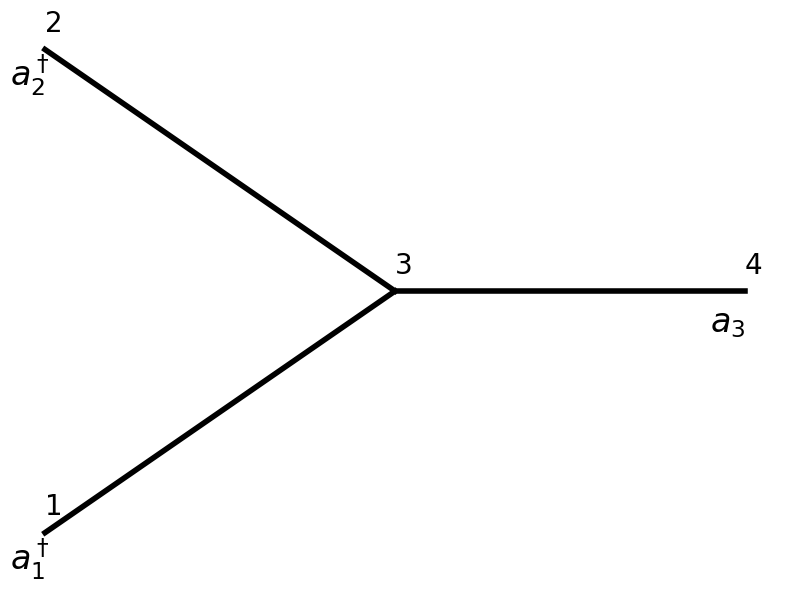
\includegraphics[width=\textwidth]{plots/1to2label.png}
        \caption{ }
        \label{fig:cannonical1_1}
    \end{subfigure}%
    \quad \raisebox{4.5\height}{\LARGE $+$}\quad
    \begin{subfigure}[t]{0.33\textwidth}
        \centering
        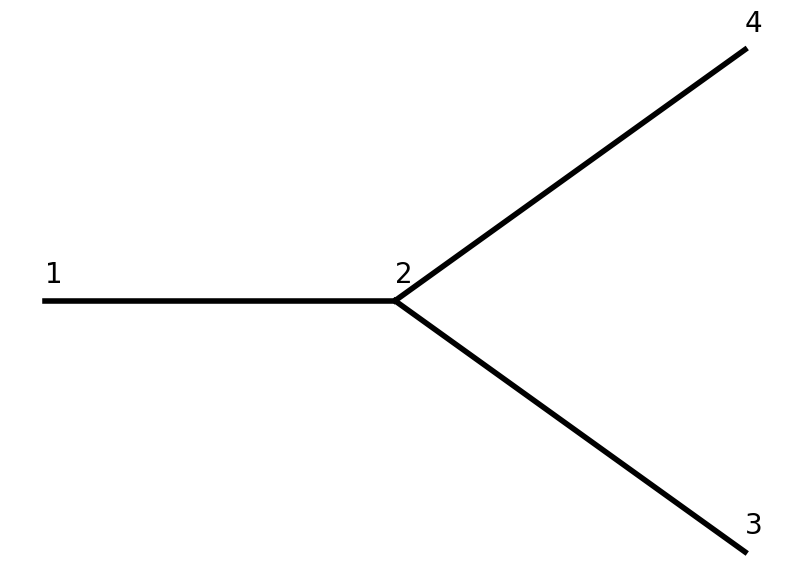
\includegraphics[width=\textwidth]{plots/2to1label.png}
        \caption{ }
        \label{fig:cannonical1_2}
    \end{subfigure}
    \caption{Canonical diagrams that go with $g$.}
    \label{fig:cannonical1}
\end{figure*}

While the term $H_{A^4}$ and $H_{\sbrackets{\partial A A}^2}$
are second order term, since they contain $g^2$ to the second power, and two structure constants.
The
diagrams obtained are shown in figures \ref{fig:cannonical2_1to3},
\ref{fig:cannonical2_3to1} and \ref{fig:cannonical2_2to2}. Each of these diagrams
corresponds to a different term in the Hamiltonian, contributing to different processes.

\begin{figure*}[h!]
    \centering
    \begin{subfigure}[t]{0.33\textwidth}
        \centering
        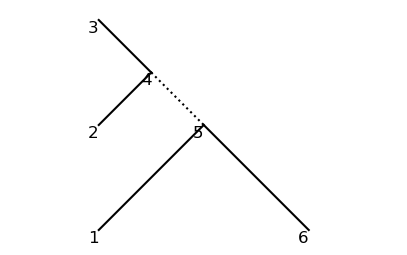
\includegraphics[width=\textwidth]{plots/canonical/order2/1.png}
        \caption{ }
    \end{subfigure}%
    \begin{subfigure}[t]{0.33\textwidth}
        \centering
        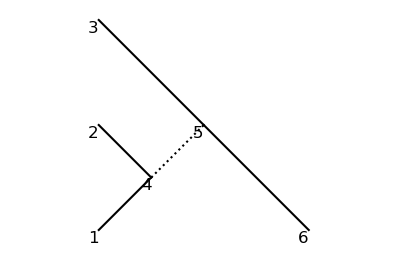
\includegraphics[width=\textwidth]{plots/canonical/order2/2.png}
        \caption{ }
    \end{subfigure}
    \begin{subfigure}[t]{0.33\textwidth}
        \centering
        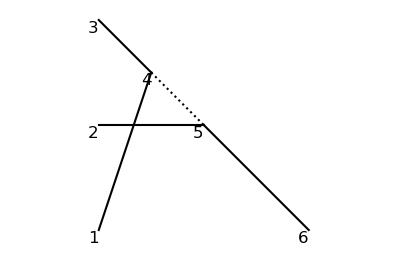
\includegraphics[width=\textwidth]{plots/canonical/order2/3.png}
        \caption{ }
    \end{subfigure}
    \caption{Canonical diagrams that go with $g^2$ in the term $\Xi_{\sbrackets{\partial AA}^2}$, 
    where one gluon is annihilated, and 3 gluons are created.}
    \label{fig:cannonical2_1to3}
\end{figure*}

\begin{figure*}[h!]
    \centering
    \begin{subfigure}[t]{0.33\textwidth}
        \centering
        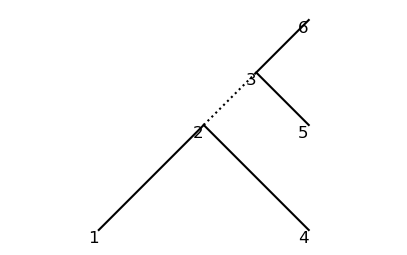
\includegraphics[width=\textwidth]{plots/canonical/order2/9.png}
        \caption{ }
    \end{subfigure}%
    \begin{subfigure}[t]{0.33\textwidth}
        \centering
        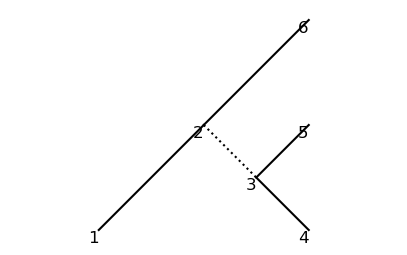
\includegraphics[width=\textwidth]{plots/canonical/order2/10.png}
        \caption{ }
    \end{subfigure}
    \begin{subfigure}[t]{0.33\textwidth}
        \centering
        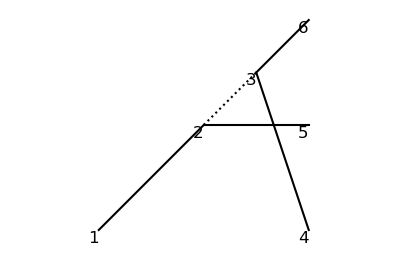
\includegraphics[width=\textwidth]{plots/canonical/order2/11.png}
        \caption{ }
    \end{subfigure}
    \caption{Canonical diagrams of order 2, for the term Hermitian conjugate with 
    coefficient 
    $\Xi_{\sbrackets{\partial AA}^2}^*$, where 3 gluons are annihilated, and
    1 gluon is created.}
    \label{fig:cannonical2_3to1}
\end{figure*}

\begin{figure*}[h!]
    \centering
    \begin{subfigure}[t]{0.24\textwidth}
        \centering
        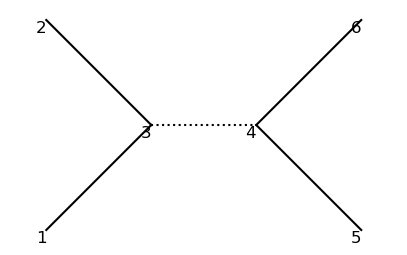
\includegraphics[width=\textwidth]{plots/canonical/order2/4.png}
        \caption{ }
    \end{subfigure}%
    \begin{subfigure}[t]{0.24\textwidth}
        \centering
        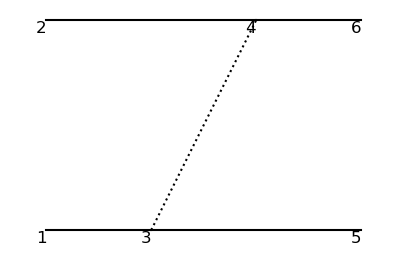
\includegraphics[width=\textwidth]{plots/canonical/order2/5.png}
        \caption{ }
    \end{subfigure}
    \begin{subfigure}[t]{0.24\textwidth}
        \centering
        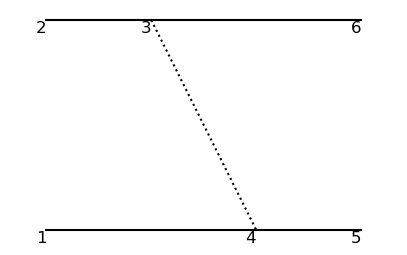
\includegraphics[width=\textwidth]{plots/canonical/order2/6.png}
        \caption{ }
    \end{subfigure}
    \begin{subfigure}[t]{0.24\textwidth}
        \centering
        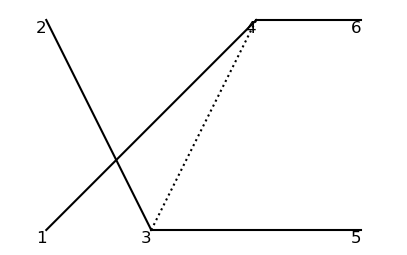
\includegraphics[width=\textwidth]{plots/canonical/order2/7.png}
        \caption{ }
    \end{subfigure}
    \begin{subfigure}[t]{0.24\textwidth}
        \centering
        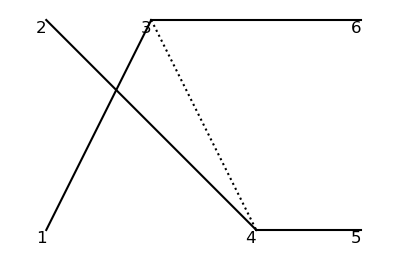
\includegraphics[width=\textwidth]{plots/canonical/order2/8.png}
        \caption{ }
    \end{subfigure}
    \caption{Canonical diagrams of order 2, for the term $X_{\sbrackets{\partial AA}^2}$, 
    where 2 gluons are annihilated, and 2 gluons are created.}
    \label{fig:cannonical2_2to2}
\end{figure*}

\begin{comment}

\subsection{Canonical diagrams}

Each of these interaction terms can be associated with a diagram representing 
annihilation and creation of particles in a vertex. They are the elementary 
objects to obtain the diagrams of higher order.

Following the creation and annihilation operators in the different terms of the 
Hamiltonian, we can distinguish the different types of process that are being
considered. 

Starting from the term $H_{A^2}$ in equation \eqref{eq:H_A^2}, we can see that this 
a particle of certain momentum $k$ is annihilated and created, producing the same
particle. This corresponds to the kinetic term of the Hamiltonian, and the diagram 
will be a line with the same color/type of particle in both ends. Since it is an 
order 0 terms, it will not contribute to the perturbative expansion.

Figure \ref{fig:cannonical1} shows the two types of first-order diagrams 
(one gluon splitting into two, and its inverse process of two gluons merging into one),
corresponding to the term $H_{A^3}$ in equation \eqref{eq:H_A^3}.
This process is represented by a diagram with 3 external legs, and 1 vertex, thus a 
first order term.

\begin{figure*}[h!]
    \centering
    \begin{subfigure}[t]{0.33\textwidth}
        \centering
        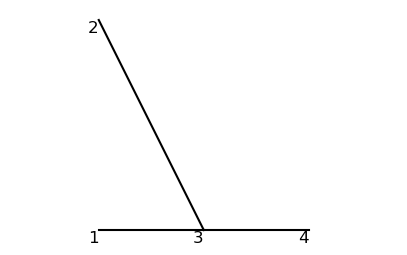
\includegraphics[width=\textwidth]{plots/canonical/order1/1.png}
        \caption{ }
    \end{subfigure}%
    \begin{subfigure}[t]{0.1\textwidth}
        \centering
        {\LARGE $+$}
    \end{subfigure}
    \begin{subfigure}[t]{0.33\textwidth}
        \centering
        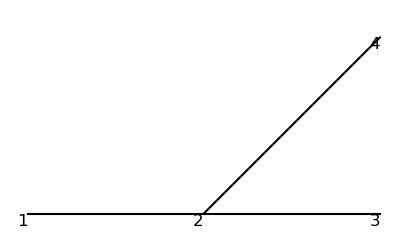
\includegraphics[width=\textwidth]{plots/canonical/order1/2.png}
        \caption{ }
    \end{subfigure}
    \caption{Canonical diagrams of order 1}
    \label{fig:cannonical1}
\end{figure*}

The term $H_{A^4}$ in equation \eqref{eq:H_A^4} is a four-gluon vertex, where either
1 gluon is annihilated, and 3 gluons are created, 3 gluons are annihilated, and
1 gluon is created, or 2 gluons are annihilated, and 2 gluons are created. However, 
since we are building higher-order diagrams from lower-order ones, it’s convenient 
to treat the four-gluon vertex as a combination of two three-gluon vertices. Meaning that 
for the process where one gluon goes to 3 gluons, we consider the process as, 
one gluon being annihilated, and 2 gluons are created, then one of the
created gluons is annihilated, and 2 gluons are created, producing a total of 3 gluons
in the final state. The same applies for the process where 3 gluons are annihilated.
This way, these diagrams have 2 vertices, and thus a second order term, that 
can be obtained from the product of the canonical first order diagrams, so we 
will not consider them as a new canonical diagrams, but rather as a result that will
be obtained during the perturbative expansion.

The $H_{\sbrackets{\partial A A}^2}$ term \eqref{eq:H_partial} represents an instantaneous gluon exchange 
(often drawn as a vertical line in light-front diagrams). This allows to consider 
processes where a gluon is annihilated, and 3 gluons are created, to a 
pair of three-gluon vertices, similar to $H_{A^4}$. The main difference is that
the interaction is instantaneous, meaning that the gluon is annihilated, and the
3 gluons are created at the same time, without any time delay between them.

In our program, we treat this as a special kind of ‘virtual particle’ (drawn with 
a dotted line) to include it in the same diagram framework. Similar to the 
term $H_{A^4}$, this term is a four-gluon vertex, except for the instantaneous 
interaction. 

The different sum terms in the equation \eqref{eq:H_partial} indicate the different 
processes that can be considered, the first term $\Xi_{\sbrackets{\partial A A}^2 1234}$
indicate the process where 1 gluon is annihilated, and 3 gluons are created, as shown in
figure \ref{fig:cannonical2_1to3}. The second term $\Xi_{\sbrackets{\partial A A}^2 1234}^*$
indicate the hermitian conjugate of the first term, where 3 gluons are annihilated, and
1 gluon is created, as shown in figure \ref{fig:cannonical2_3to1}. The third term
$X_{\sbrackets{\partial A A}^2 1234}$ indicate the process where 2 gluons are annihilated,
and 2 gluons are created, as shown in figure \ref{fig:cannonical2_2to2}.

\begin{figure*}[h!]
    \centering
    \begin{subfigure}[t]{0.33\textwidth}
        \centering
        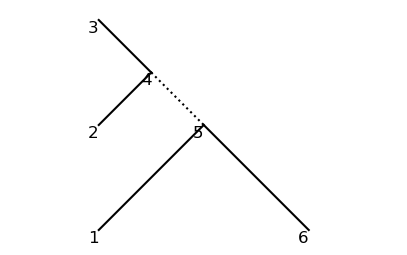
\includegraphics[width=\textwidth]{plots/canonical/order2/1.png}
        \caption{ }
    \end{subfigure}%
    \begin{subfigure}[t]{0.33\textwidth}
        \centering
        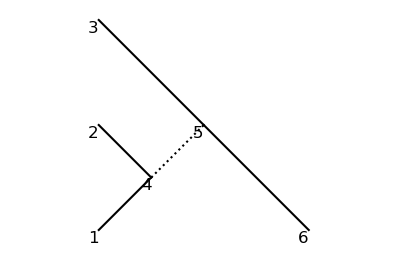
\includegraphics[width=\textwidth]{plots/canonical/order2/2.png}
        \caption{ }
    \end{subfigure}
    \begin{subfigure}[t]{0.33\textwidth}
        \centering
        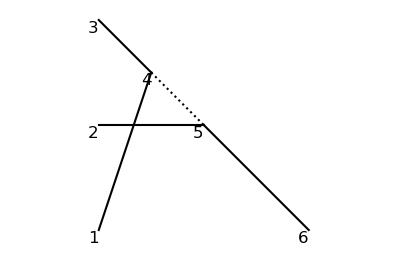
\includegraphics[width=\textwidth]{plots/canonical/order2/3.png}
        \caption{ }
    \end{subfigure}
    \caption{Canonical diagrams of order 2, for the term $\Xi_{\sbrackets{\partial AA}^2}$, 
    where one gluon is annihilated, and 3 gluons are created.}
    \label{fig:cannonical2_1to3}
\end{figure*}

\begin{figure*}[h!]
    \centering
    \begin{subfigure}[t]{0.33\textwidth}
        \centering
        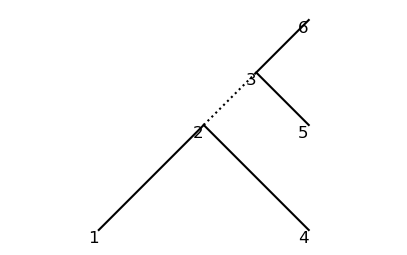
\includegraphics[width=\textwidth]{plots/canonical/order2/9.png}
        \caption{ }
    \end{subfigure}%
    \begin{subfigure}[t]{0.33\textwidth}
        \centering
        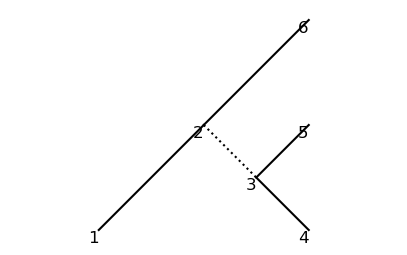
\includegraphics[width=\textwidth]{plots/canonical/order2/10.png}
        \caption{ }
    \end{subfigure}
    \begin{subfigure}[t]{0.33\textwidth}
        \centering
        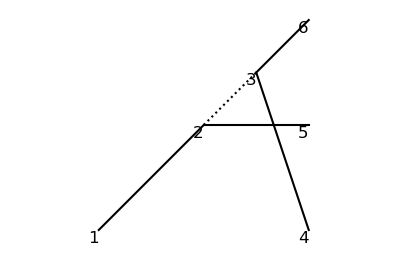
\includegraphics[width=\textwidth]{plots/canonical/order2/11.png}
        \caption{ }
    \end{subfigure}
    \caption{Canonical diagrams of order 2, for the term hermitian conjugate of 
    $\Xi_{\sbrackets{\partial AA}^2}$, where 3 gluons are annihilated, and
    1 gluon is created.}
    \label{fig:cannonical2_3to1}
\end{figure*}

\begin{figure*}[h!]
    \centering
    \begin{subfigure}[t]{0.24\textwidth}
        \centering
        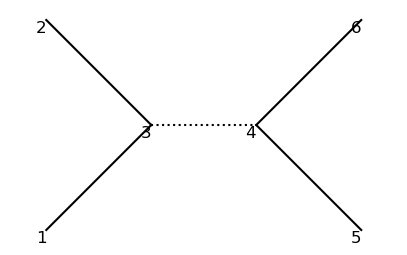
\includegraphics[width=\textwidth]{plots/canonical/order2/4.png}
        \caption{ }
    \end{subfigure}%
    \begin{subfigure}[t]{0.24\textwidth}
        \centering
        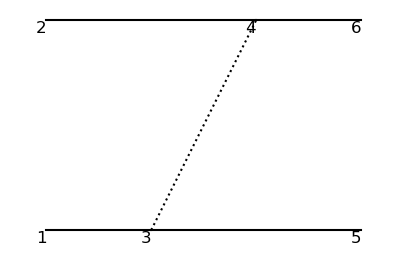
\includegraphics[width=\textwidth]{plots/canonical/order2/5.png}
        \caption{ }
    \end{subfigure}
    \begin{subfigure}[t]{0.24\textwidth}
        \centering
        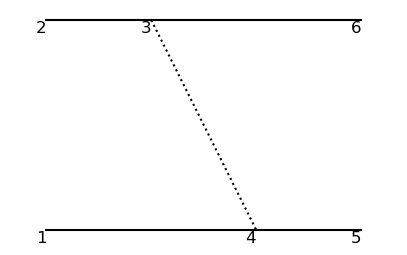
\includegraphics[width=\textwidth]{plots/canonical/order2/6.png}
        \caption{ }
    \end{subfigure}
    \begin{subfigure}[t]{0.24\textwidth}
        \centering
        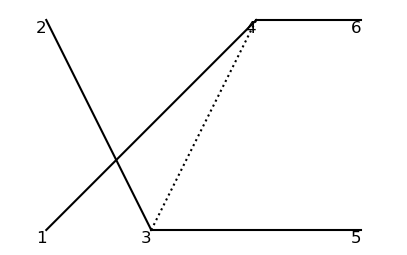
\includegraphics[width=\textwidth]{plots/canonical/order2/7.png}
        \caption{ }
    \end{subfigure}
    \begin{subfigure}[t]{0.24\textwidth}
        \centering
        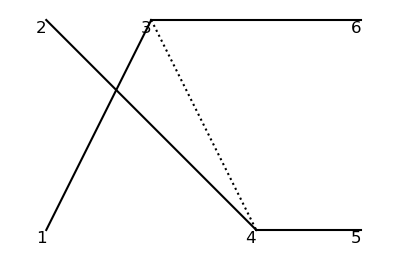
\includegraphics[width=\textwidth]{plots/canonical/order2/8.png}
        \caption{ }
    \end{subfigure}
    \caption{Canonical diagrams of order 2, for the term $X_{\sbrackets{\partial AA}^2}$, 
    where 2 gluons are annihilated, and 2 gluons are created.}
    \label{fig:cannonical2_2to2}
\end{figure*}

\newpage

The combination of all these diagrams, are the canonical diagrams of order 2.
Together with the diagrams of order 1, figure \ref{fig:cannonical1},
they form the basis of the perturbative expansion of the Hamiltonian, and the
starting point to obtain the diagrams of higher order.

\end{comment}

\newpage

\subsection{Renormalization group procedure for effective particles (RGPEP)}
\label{sec:rgpep}
The RGPEP, is a renormalization group procedure applied within the Hamiltonian formulation 
of quantum field theory, formulated by S.D.Głazek and K.G.Wilson \cite{Glazek:1997gt,Wilson:1994fk,Glazek:1994qc,PhysRevD.48.5863}. 
By considering a series of unitary transformations applied to the
canonical or bare Hamiltonian, the RGPEP is able to construct a succession of effective 
Hamiltonians $\mathcal{H}_s$, each describing dynamics in terms of effective particles 
at a resolution scale set by the parameter~\( s \). This is associated with the 
renormalization group scale $\lambda = 1/s$, where $\lambda$ has dimension of energy,
and has the interpretation of the characteristic energy scale of the theory, 
while \( s \) has dimension of length, and has the interpretation of the 
\textit{size} of effective particles.

Effective particles, are defined by effective-particle 
operators that differs from the canonical ones by the unitary transformation 
$\mathcal{U}_s$,

\begin{equation}
    a_s = \mathcal{U}_sa_0\mathcal{U}_s^\dagger.
    \label{eq:effective_particle_operator}
\end{equation}

Due to dimensional and notational reasons, it is convenient to consider the scale 
parameter $t = s^4$ instead.

Then, for $s=0$ or, equivalently, $t=0$, the theory describes  point-like or bare particles, 
those associated to the canonical Hamiltonian $\mathcal{H}_0(a_0)$.

The effective Hamiltonian $\mathcal{H}_t$, written in terms of the effective particle
operator $a_s$, is related to the regulated canonical Hamiltonian with counter-terms 
by the condition (section \ref{sec:regulatrization_countertems}),

\begin{equation}
    \mathcal{H}_t(a_t) = \mathcal{H}_0(a_0),
\end{equation}

Using Eq.~\eqref{eq:effective_particle_operator} and expressing all operators in 
terms of the original \( a_0 \), the effective Hamiltonian becomes,

\begin{equation}
    \mathcal{H}_t(a_0) = \mathcal{U}_t^\dagger\mathcal{H}_0(a_0) \mathcal{U}_t.
\end{equation}

Differentiating with respect of $t$, one obtains the RGPEP differential equation,

\begin{equation}
    \mathcal{H}_t^\prime (a_0) = \frac{d}{dt}\mathcal{H}_t(a_0) = 
    \sbrackets{-\mathcal{U}_t^\dagger \mathcal{U}_t^\prime, \mathcal{H}_t(a_0)} 
    \equiv \sbrackets{\mathcal{G}_t(a_0), \mathcal{H}_t(a_0)},
\end{equation}
where $\mathcal{G}_t$ is the generator of the RGPEP transformation. 

Considering the generator from Ref. \cite{PEP},
\begin{equation}
    \mathcal{G}_t = \sbrackets{\mathcal{H}_f, \mathcal{H}_{Pt}},
\end{equation}
where $\mathcal{H}_f$ is the free part of $\mathcal{H}_t$ and does not depend on 
the coupling constant \( g \), 
while $\mathcal{H}_{Pt}$ is defined as $\mathcal{H}_t$ but contains a kinematical factor
depending on momenta of particle involved.

The resulting RGPEP equation has the form,
\begin{equation}
    \mathcal{H}_t^\prime =  \sbrackets{\sbrackets{\mathcal{H}_f, \mathcal{H}_{Pt}}, \mathcal{H}_t}.
\end{equation}

Constructing an effective Hamiltonian using RGPEP amounts to solving this equation.

In general, the solution of the RGPEP equation is a non-trivial task, and a perturbative
expansion of the effective Hamiltonian is used, expressing  
$\mathcal{H}_t$ as a power series of the coupling constant $g$,

\begin{equation}
    \mathcal{H}_t = \sum_{n=0}^{\infty} g^n \mathcal{H}_{t n} = 
    \mathcal{H}_{0} + g \mathcal{H}_{t 1} + g^2 \mathcal{H}_{t 2} + g^3 \mathcal{H}_{t 3} +
    g^4 \mathcal{H}_{t 4} + \cdots.
\end{equation}

Substituting into the RGPEP equation, and collecting terms order by order in \( g \),
the following system of coupled first-order differential equations is obtained,
\begin{align}
        \mathcal{H}_{0}^\prime &= 0, \label{eq:diff_order0}\\
        g\mathcal{H}_{t 1}^\prime &= \sbrackets{\sbrackets{\mathcal{H}_0, g\mathcal{H}_{Pt 1}}, 
        \mathcal{H}_{0}}, \label{eq:diff_order1}\\
        g^2\mathcal{H}_{t 2}^\prime &= \sbrackets{\sbrackets{\mathcal{H}_0, g^2\mathcal{H}_{Pt 2}}, 
        \mathcal{H}_{0}} + \sbrackets{\sbrackets{\mathcal{H}_0, g\mathcal{H}_{Pt 1}}, 
        g\mathcal{H}_{t 1}}, \\
        g^3\mathcal{H}_{t 3}^\prime &= \sbrackets{\sbrackets{\mathcal{H}_0, g^3\mathcal{H}_{Pt 3}}, 
        \mathcal{H}_{0}} + \sbrackets{\sbrackets{\mathcal{H}_0, g^2\mathcal{H}_{Pt 2}}, 
        g\mathcal{H}_{t 1}} + \sbrackets{\sbrackets{\mathcal{H}_0, g\mathcal{H}_{Pt 1}}, 
        g^2\mathcal{H}_{t 2}}. \label{eq:diff_order3}\\
        &\vdots \nonumber
\end{align}

The order 0 term is trivially solvable from an initial condition, and the solution of the 
equation of order 1 will be an exponential of the parameter $t$ times the initial condition $\mathcal{H}_{01}$. The 2nd order 
solution can be obtained from 1th order, and the 3rd order from the previous orders, 
and so on. At this point, the use of diagrams becomes crucial.


\subsubsection{Regularization and Counterterms}\label{sec:regulatrization_countertems}

In QCD, the bare Hamiltonian is ill-defined due to the presence of elements 
that contain ultraviolet (UV) divergences and infrared (IR) divergences
\cite{QCDG,glazek_renormalization_1993}.
The UV divergences are produced in processes involving large momentum transfers, 
whereas the IR divergences occur in processes with ‘soft’ particles carrying small 
longitudinal momentum fractions, $x_{p/P} = p^+/P^+$, yielding zeros in  
denominators.

To deal with these divergences a regulating factor $r$ is 
introduced in every interacting term. These factors make the interacting terms rapidly 
tend to zero, if the change in the transverse momentum of any gluon exceeds a certain
cutoff parameter $\Delta$, or if the change in longitudinal momentum of any gluon is
greater than a cutoff parameter $\delta$ \cite{Collins_1984}. 


The particle operators are multiplied by the regulating factor, 
\begin{equation}
    r_{\Delta \delta} (k^\perp, x) = r_\Delta (k^\perp) r_\delta(x).
\end{equation}

The transverse regulator factor, $r_\Delta (k^\perp)$ will ensure that UV processes are suppressed.
And the longitudinal regulator factor $r_\delta(x)$ must verify a similar condition, preventing terms
of the form $1/x$ or $1/x^2$ to blow up as $x$ approaches 0. 

The exact form of the regulator factors is not important for our purposes, as long as it 
verifies the condition, since it will be removed once we take the
limit $\Delta \to \infty$ and $\delta \to 0$.


The counterterms are an additional term added to the initial or bare Hamiltonian 
$\mathcal{H}_0$ to deal with divergent integrals. 

They are defined in a way, such that the coefficients of products 
of creation and annihilation operators in the effective theory for gluons of size $s$
become independent of the regularization parameter $\Delta$ when the regularization
in dynamics of gluons of size zero is being removed. The rest of the unknown parts 
of the counterterms are adjusted to respect the symmetries of the theory, and must 
match the predictions of the theory with the experimental results.

The distinction between regularization and counterterms may be confusing, but the
regularization is a procedure to prevent the divergences that arise
in the theory, while the counterterms are the terms added to the Hamiltonian to 
cancel the dependency on such regulators, so that after the cutoffs are removed, the 
effective Hamiltonian remains finite and regulator independent. Regularization is
an essential first step in the renormalization process.

\subsubsection{Order by order solutions.} \label{sec:orderbyorder_solutions}

The solution of the differential equations \eqref{eq:diff_order1} to \eqref{eq:diff_order3} 
and so on, without considering the RGPEP factors resulting from integration that would multiply each term.

\begin{align}
    \mathcal{H}_{t1} & = f_{t} \mathcal{H}_{01} \\
    \mathcal{H}_{t2} & \sim \mathcal{H}_{02} + \mathcal{H}_{01} 
    \mathcal{H}_{01}\\
    \mathcal{H}_{t3} & \sim \mathcal{H}_{03} + \mathcal{H}_{01} \mathcal{H}_{01}
    \mathcal{H}_{01} + \parenthesis{\mathcal{H}_{02} \mathcal{H}_{01} + 
    \mathcal{H}_{01} \mathcal{H}_{02}}\\
    \mathcal{H}_{t4} & \sim \mathcal{H}_{04} + \mathcal{H}_{01} \mathcal{H}_{01}
    \mathcal{H}_{01} \mathcal{H}_{01} + \parenthesis{\mathcal{H}_{02} 
    \mathcal{H}_{01} \mathcal{H}_{01} +  \mathcal{H}_{01} \mathcal{H}_{02}
    \mathcal{H}_{01} + \mathcal{H}_{01} \mathcal{H}_{01} \mathcal{H}_{02}} \nonumber\\
    & + \parenthesis{\mathcal{H}_{03} \mathcal{H}_{01} + \mathcal{H}_{01} 
    \mathcal{H}_{03} + \mathcal{H}_{02}\mathcal{H}_{02}},\\
    &\vdots  \nonumber
\end{align}
where $f_{t}$ is a form factor that depends on the scale $t$ which has the form
of an exponential that
results from the first-order equation.
Such form factor suppresses the transition between states with 
different invariant mass.

Integrating order by order, additional factors are obtained. But they are ignored
in this analysis and replaced by the symbol "$\sim$" to focus on structure 
resulting from the product of interactions.

This shows how an iterative 
process can be used to obtain the solution for each order.

The first-order diagrams are simply the canonical diagrams, with one power of $g$ 
and denoted by $\mathcal{H}_{01}$. 

As for the second order, 
they contain the canonical diagrams with power $g^2$, and the counterterms,
all together $\mathcal{H}_{02}$, and the product of 2 first-order diagrams. 

The 
third order contains only the counterterms from the third order $\mathcal{H}_{03}$,
the product of the first order, and second order canonical diagrams, as well as the 
product of exclusive first order diagrams.

\newpage


\section{Code implementation} \label{sec:code}

The code is implemented in Python, but the principles of the method can be written in any 
programming language. The program is designed to be modular, and applicable to any
other theory. These require changing the canonical
diagrams. These modifications are beyond the scope of this work, and they are not presented
here explicitly.


\subsection{Diagram representation}

Every term in the Hamiltonian can be identified with a diagram, according to the 
structure of the creation and annihilation operators present in it.
The time order of the interaction is very important. In our convention, the time flows from right to left.

Each diagram 
will be composed of different elements:

\begin{itemize}
    \item \textbf{External legs}: representation of the incoming and outgoing particles or 
    the annihilation and creation operators, respectively. They determine the type 
    of interaction that is being considered. (e.g. in figure \ref{fig:loop_example},
    the connection of points [1, 2] or [3, 4] are external legs of the diagram.)
    \item \textbf{Internal legs}: represent the virtual particles that are exchanged during the
    process, or the intermediate creation and annihilation operators that are 
    eliminated in the normal-ordering process. These creation and annihilation operators
    are not present in the effective Hamiltonian. (e.g. in figure \ref{fig:loop_example},
    the 2 connection from [2, 3] are the internal legs of the diagram.)
    \item \textbf{Vertices}: points where interactions between particles occur, the number of
    vertices in a diagram indicates the order at which the diagram is contributing. 
    (e.g. in figure \ref{fig:loop_example}, the points 1, 2, ... are the vertices
    of the diagram.)
    \item \textbf{Loops}: closed paths in the diagrams, formed by the internal legs. In 
    general, they are divergent terms. Example in figure \ref{fig:loop_example}.
    \begin{figure}[h!]
        \centering
        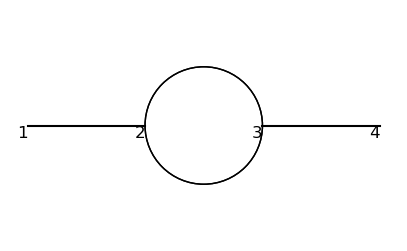
\includegraphics[width=0.5\textwidth]{plots/order2/from_order1/3.png}
        \caption{Example of a loop in a diagram, formed by the internal legs.}
        \label{fig:loop_example}
    \end{figure}
    \item \textbf{Counterterms} additional terms added to the Hamiltonian to deal with the divergences
    produced during the process. These will be represented with a dot in the diagram.
\end{itemize}

Notice that the diagrams are different from the well-known Feynman diagrams\cite{Peskin:1995ev}.
The essential difference is the importance of the order of appearance
of the interactions. Altering
the order of the vertices in the diagram will produce a different interaction terms. 

As another example, consider the diagrams in figure \ref{fig:example_diagram}, this pair of 
diagrams are contributions to the three-gluon vertex (one gluon yielding two gluons), 
with the counterterm associated with it. 

\begin{figure*}[h!]
    \centering
    \begin{subfigure}[t]{0.5\textwidth}
        \centering
        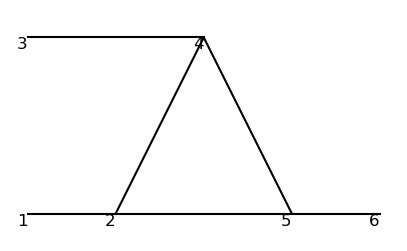
\includegraphics[width=0.7\textwidth]{plots/order3/order3_1to2/1.png}
        \caption{Diagram with a three-gluon loop.}
        \label{fig:example_diagram_1}
    \end{subfigure}%
    \begin{subfigure}[t]{0.5\textwidth}
        \centering
        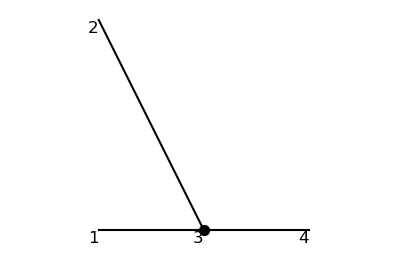
\includegraphics[width=0.7\textwidth]{plots/order3/order3_1to2/counterterms/1.png}
        \caption{Counterterm of order 3 for the diagram (a)}
    \end{subfigure}
    \caption{A example of a third order contribution to the 
    process of three-gluon vertex, 1 gluon incoming and 2 gluons outgoing. (Outputs of 
    the programs.)}
    \label{fig:example_diagram}
\end{figure*}

Following the previous definitions, the diagram (figure \ref{fig:example_diagram_1}) represents
a third order interaction with a three-gluon loop: 2 gluons are 
produced in the final state from one in the intial state. Due to the presence of a loop, the diagram is
divergent, and a counterterm diagram is needed to deal with the divergence. This 
diagram is represented with a dot at the position of the loop, with the same 
external legs as the original diagram (figure \ref{fig:example_diagram}). 


\subsection{Definition of diagrams}

The diagrams are defined by 2 arrays, 
\begin{itemize}
    \item Points: arrays of dimension $N \times 2$, where $N$ is the number of 
    points in the diagram, each point is defined by its coordinates $(x,y)$.
    \item Paths: arrays of dimension $M \times N^\prime \times 2$, where $M$ is the
    number of different types of particles to consider in the theory, $N^\prime$ 
    is the number of paths for each types of particle in the diagram, and $2$ indicates
    the points to connect.
\end{itemize}

An example of the different elements can be seen in figure \ref{fig:diagram_representation}.

\begin{figure}[h!]
    \centering
    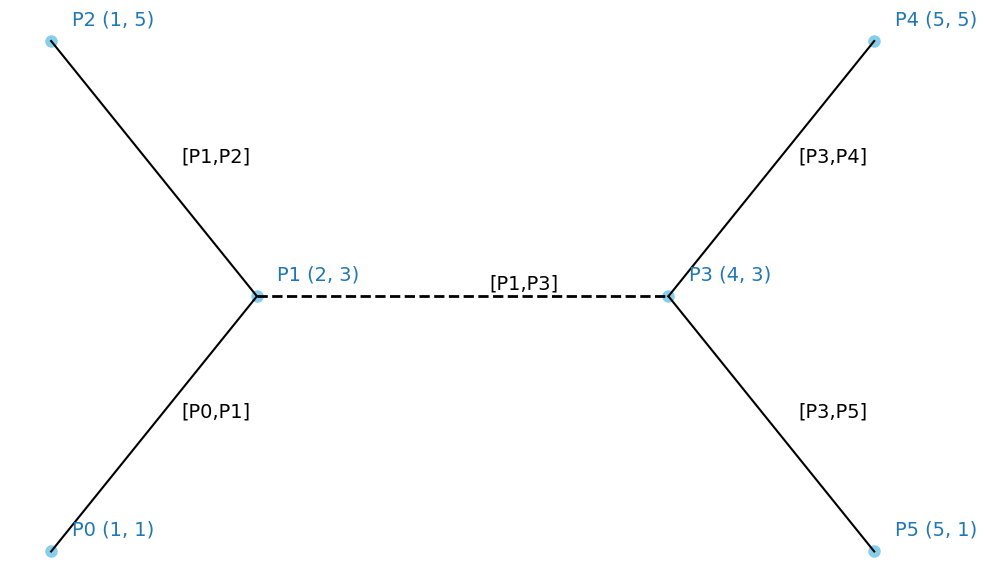
\includegraphics[width=0.7\textwidth]{plots/graph_example.png}
    \caption{Representation of a diagram as a graph, where the blue points are the $N$ points
    defined in the program, the different line-style represent the different types of particles 
    $M$, and the labels associated with each line the $N^\prime$ connections 
    for each type of particle.}
    \label{fig:diagram_representation}
\end{figure}


In the case of gluon interactions, although only 1 type of particle is present, the
instantaneous interactions have to be considered. This is done by defining this 
interaction as a new type of virtual particle in the program.

\subsection{Order by order procedure}

To calculate the diagram representing a certain order-term, the code follows the 
procedure described in Section \ref{sec:orderbyorder_solutions}. Having the
canonical diagrams as an input, the program aims to obtain all possible diagrams of such order
that contribute to a certain effective interaction, and discards those diagrams, with
different structure.

The program follows a recursive procedure, where the diagrams of order $n$ are
obtained from the diagrams of order lower orders, in a process that can be outlines
as follows,

\begin{enumerate}
    \item Start with the canonical diagrams of order 1 and 2.
    \item For each order $n$, do the following,
    \begin{enumerate}
        \item Generate all possible combinations of diagrams of lower orders, that 
        sum to the order $n$.
        \item For each combination, check if it is a valid diagram \footnote{A ‘valid’ diagram here means that the external legs of the combined diagram match the intended process. For instance, if we are interested in the 1→2 gluon process, any combination that results in a different incoming/outgoing particle count would be discarded.} 
        for the type of interaction
        being considered.
        \item If it is a valid diagram, add it to the list of diagrams for order $n$.
    \end{enumerate}
    \item After generating all the diagrams of order $n$, check for equivalent diagrams,
    and add their contributions to the list of diagrams.
    \item Check for loops, and add the counterterms for each order and process
    to the list of diagrams,
    \item Repeat the process for the next order, until the desired order is reached.
\end{enumerate}

The step 3 is fundamental in order to reduce the number of diagrams that needs to 
be used to calculate the next order. This procedure is the most time-consuming process 
of the program, needing a search algorithm to find the equivalent diagrams, meaning 
that as the order increases, the number of diagrams increases exponentially, and the 
time to find the equivalent diagrams increases exponentially too. 

To understand the process, let's consider the first iteration of the program, to calculate
the diagrams of order 2, starting from the canonical diagrams of order 1.

\begin{figure*}[h!]
  \centering
  % switch into math mode, start a stretchy left parenthesis
  $\displaystyle \mathcal{H}_{01}\mathcal{H}_{01} = 
    \left(
      % now vcenter the whole block so its height is taken into account
      \vcenter{%
        \hbox{%  
          % first subfigure
          \begin{subfigure}[t]{.08\textwidth}
            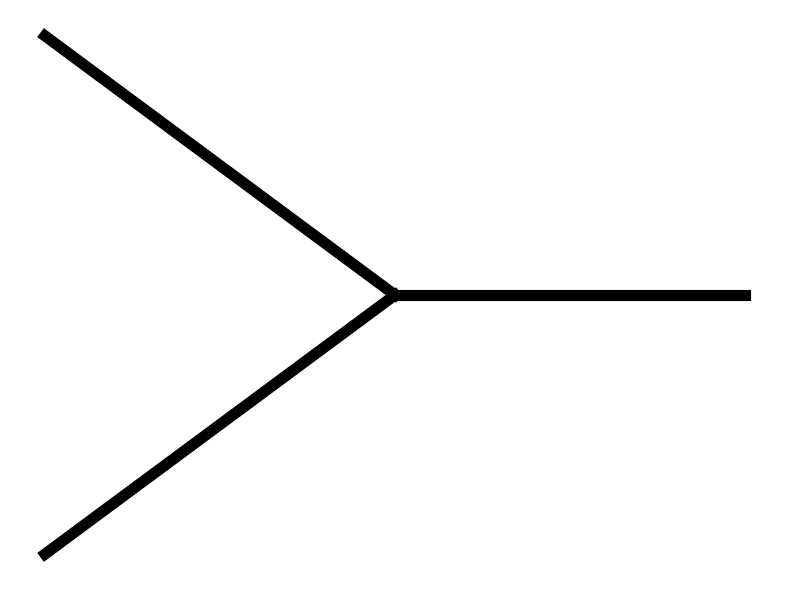
\includegraphics[width=\textwidth]{plots/1to2.png}
          \end{subfigure}%
          \quad % space between
          \raisebox{0.9\height}{\LARGE $+$}\quad
          % second subfigure
          \begin{subfigure}[t]{.08\textwidth}
            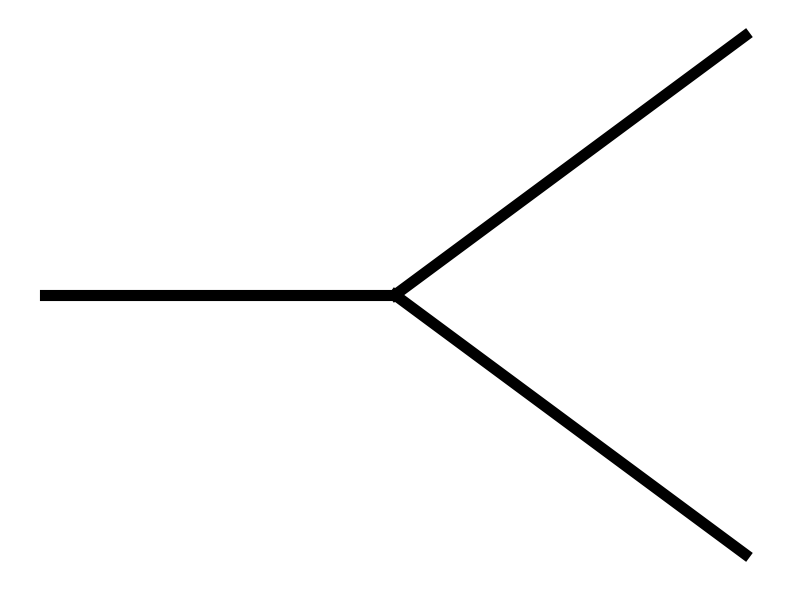
\includegraphics[width=\textwidth]{plots/2to1.png}
          \end{subfigure}%
        }% end \hbox
        }% end \vcenter
    \right)$ 
    $\displaystyle
    \left(
      % now vcenter the whole block so its height is taken into account
      \vcenter{%
        \hbox{%  
          % first subfigure
          \begin{subfigure}[t]{.08\textwidth}
            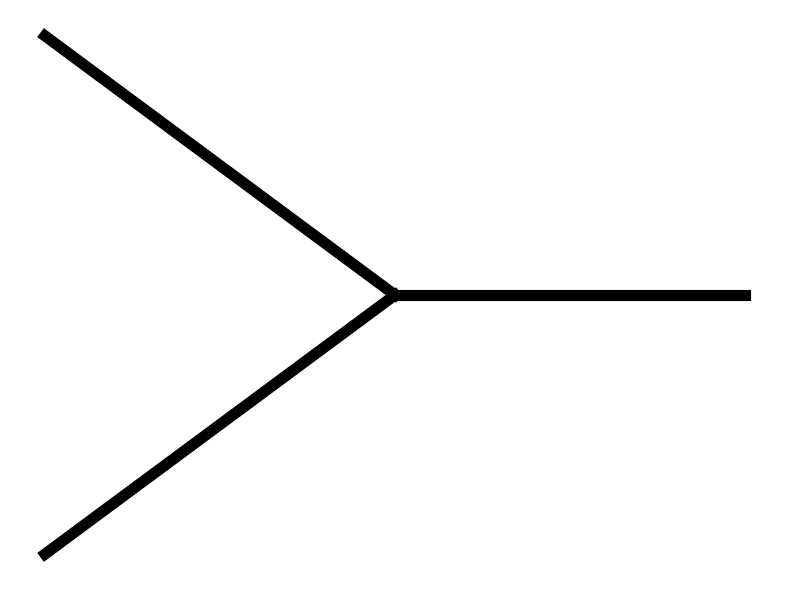
\includegraphics[width=\textwidth]{plots/1to2.png}
          \end{subfigure}%
          \quad % space between
          \raisebox{0.9\height}{\LARGE $+$}\quad
          % second subfigure
          \begin{subfigure}[t]{.08\textwidth}
            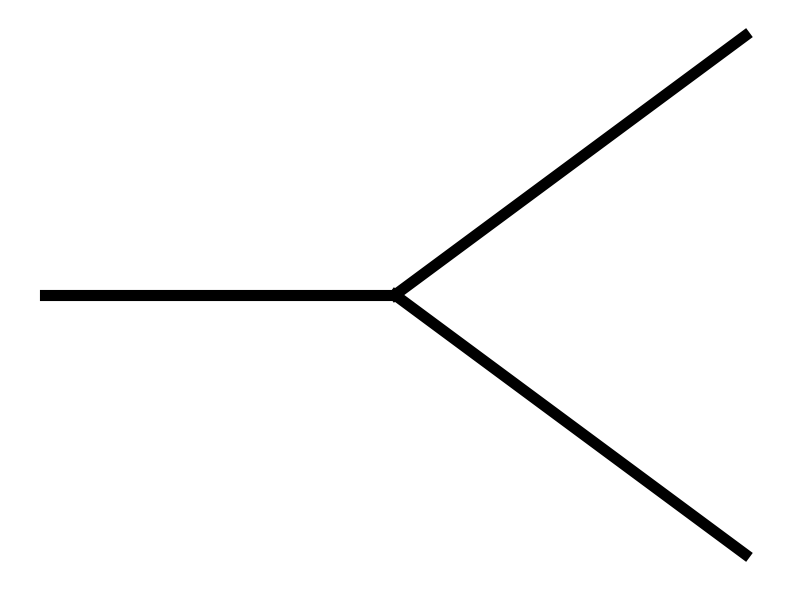
\includegraphics[width=\textwidth]{plots/2to1.png}
          \end{subfigure}%
        }% end \hbox
        }% end \vcenter
    \right) = $ 
\end{figure*}~
\begin{figure*}[h!]
  \centering
  % switch into math mode, start a stretchy left parenthesis
  $\displaystyle = 
    \left(
      % now vcenter the whole block so its height is taken into account
      \vcenter{%
        \hbox{%  
          % first subfigure
          \begin{subfigure}[t]{.08\textwidth}
            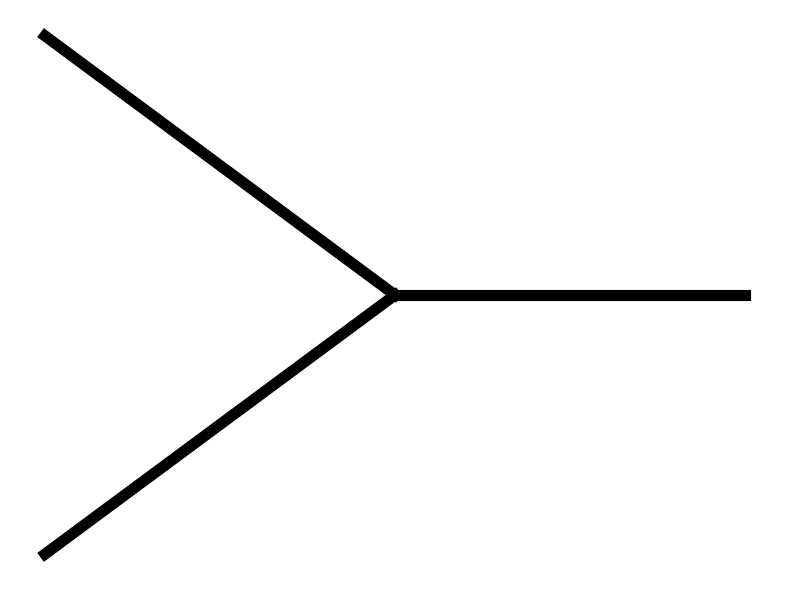
\includegraphics[width=\textwidth]{plots/1to2.png}
          \end{subfigure}%
          \begin{subfigure}[t]{.08\textwidth}
            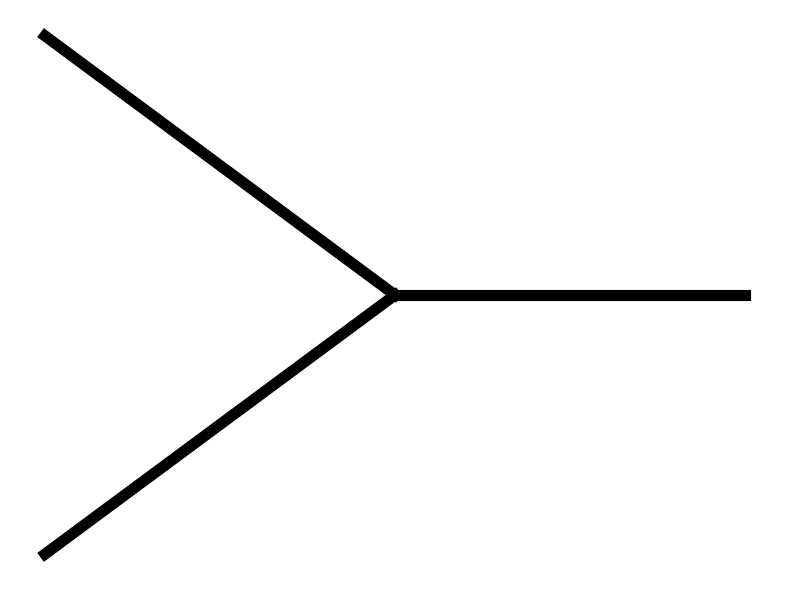
\includegraphics[width=\textwidth]{plots/1to2.png}
          \end{subfigure}%
          \quad % space between
          \raisebox{0.9\height}{\LARGE $+$}\quad
          \begin{subfigure}[t]{.08\textwidth}
            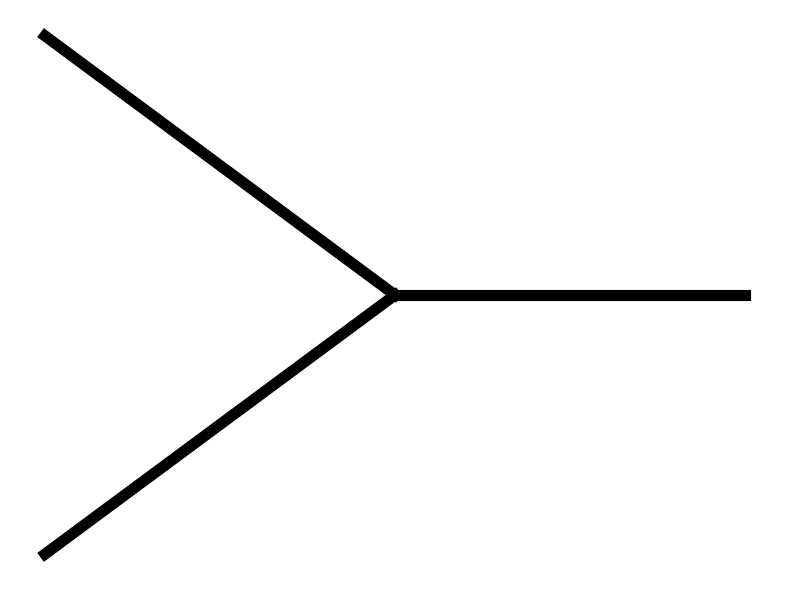
\includegraphics[width=\textwidth]{plots/1to2.png}
          \end{subfigure}%
          % second subfigure
          \begin{subfigure}[t]{.08\textwidth}
            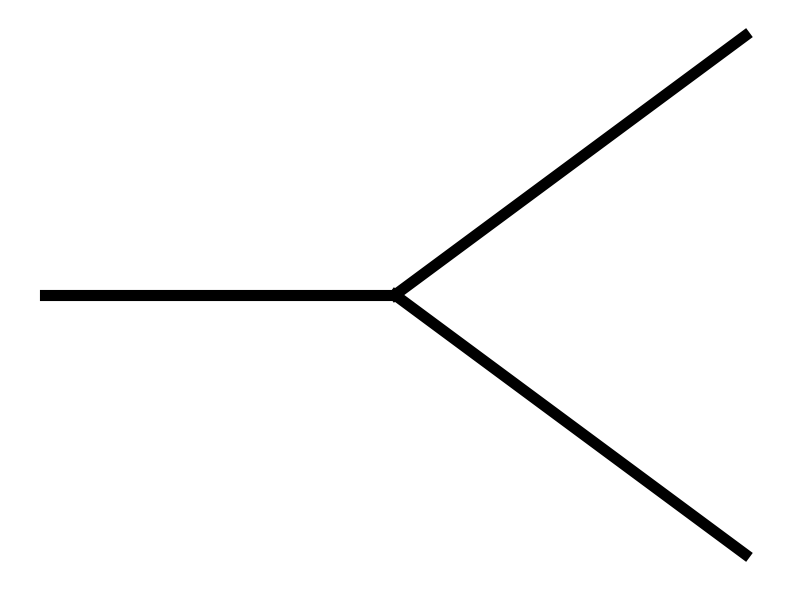
\includegraphics[width=\textwidth]{plots/2to1.png}
          \end{subfigure}%
                    \quad % space between
          \raisebox{0.9\height}{\LARGE $+$}\quad
          \begin{subfigure}[t]{.08\textwidth}
            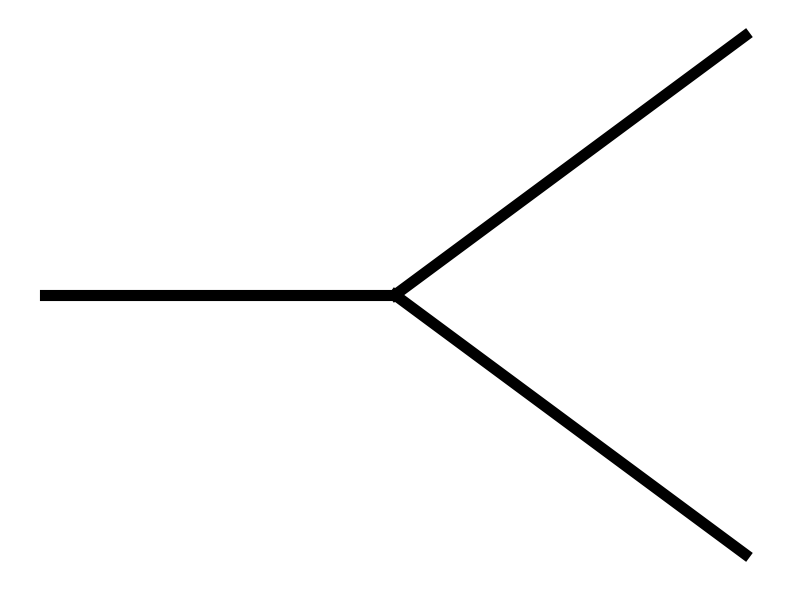
\includegraphics[width=\textwidth]{plots/2to1.png}
          \end{subfigure}%
          % second subfigure
          \begin{subfigure}[t]{.08\textwidth}
            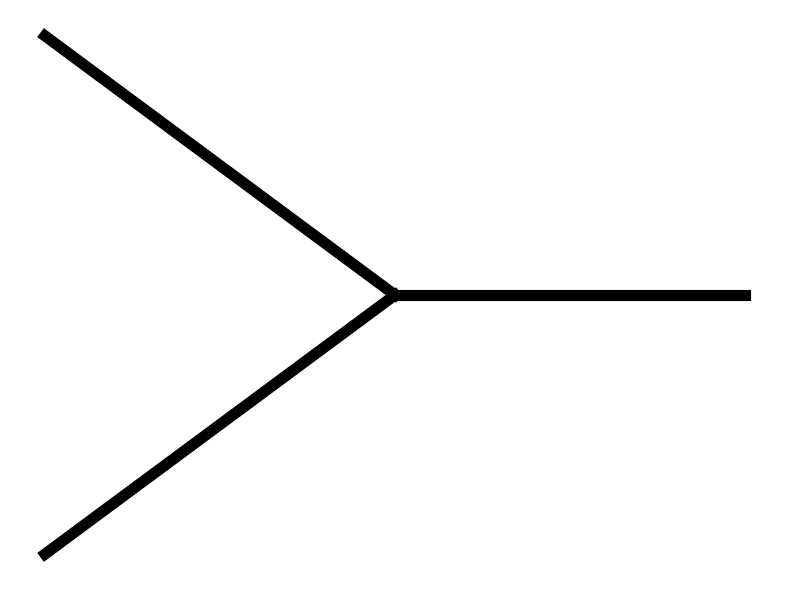
\includegraphics[width=\textwidth]{plots/1to2.png}
          \end{subfigure}%
                    \quad % space between
          \raisebox{0.9\height}{\LARGE $+$}\quad
          \begin{subfigure}[t]{.08\textwidth}
            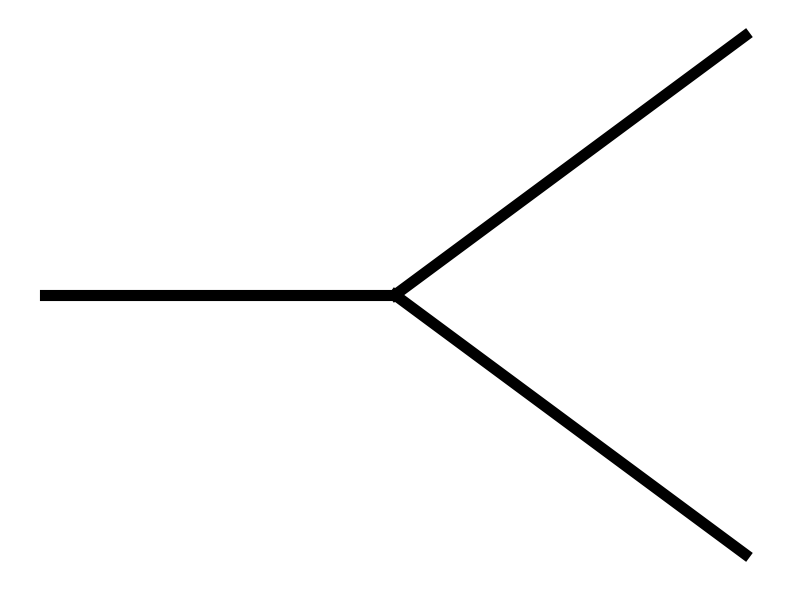
\includegraphics[width=\textwidth]{plots/2to1.png}
          \end{subfigure}%
          % second subfigure
          \begin{subfigure}[t]{.08\textwidth}
            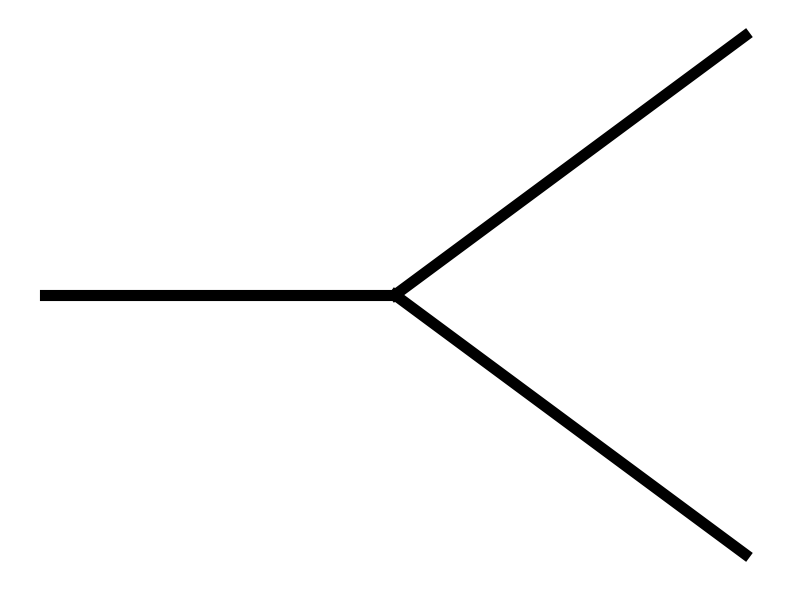
\includegraphics[width=\textwidth]{plots/2to1.png}
          \end{subfigure}%
        }% end \hbox
        }% end \vcenter
    \right)$ 
\end{figure*}

Here each term will contribute at second-order to a different type of interaction.
For instance, the first term will contribute to the process of 1 gluon going to 3 gluons,
since one of the outgoing gluon from the second diagram will "connect" to the incoming gluon
of the first diagram. Due to 2 possible connections, this term produces 2 equivalent diagrams.

\begin{figure*}[h!]
  \centering
  % switch into math mode, start a stretchy left parenthesis 
    % first subfigure
    \begin{subfigure}[t]{.1\textwidth}
    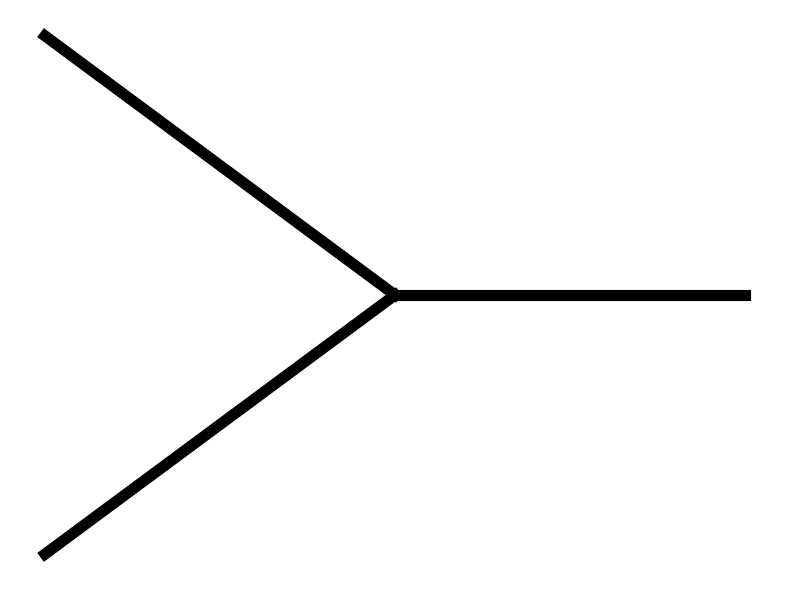
\includegraphics[width=\textwidth]{plots/1to2.png}
    \end{subfigure}%
    \begin{subfigure}[t]{.1\textwidth}
    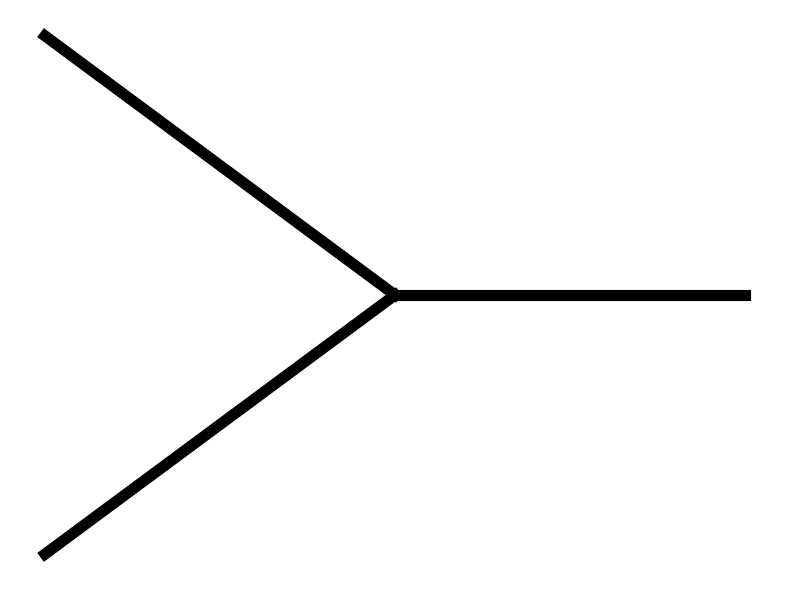
\includegraphics[width=\textwidth]{plots/1to2.png}
    \end{subfigure}%
    $\displaystyle \quad % space between
    \raisebox{1.8\height}{\LARGE $\to$}\quad $
    $\displaystyle \quad % space between
    \raisebox{1.2\height}{\Large $2\quad\cdot$} $
    \begin{subfigure}[t]{.2\textwidth}
    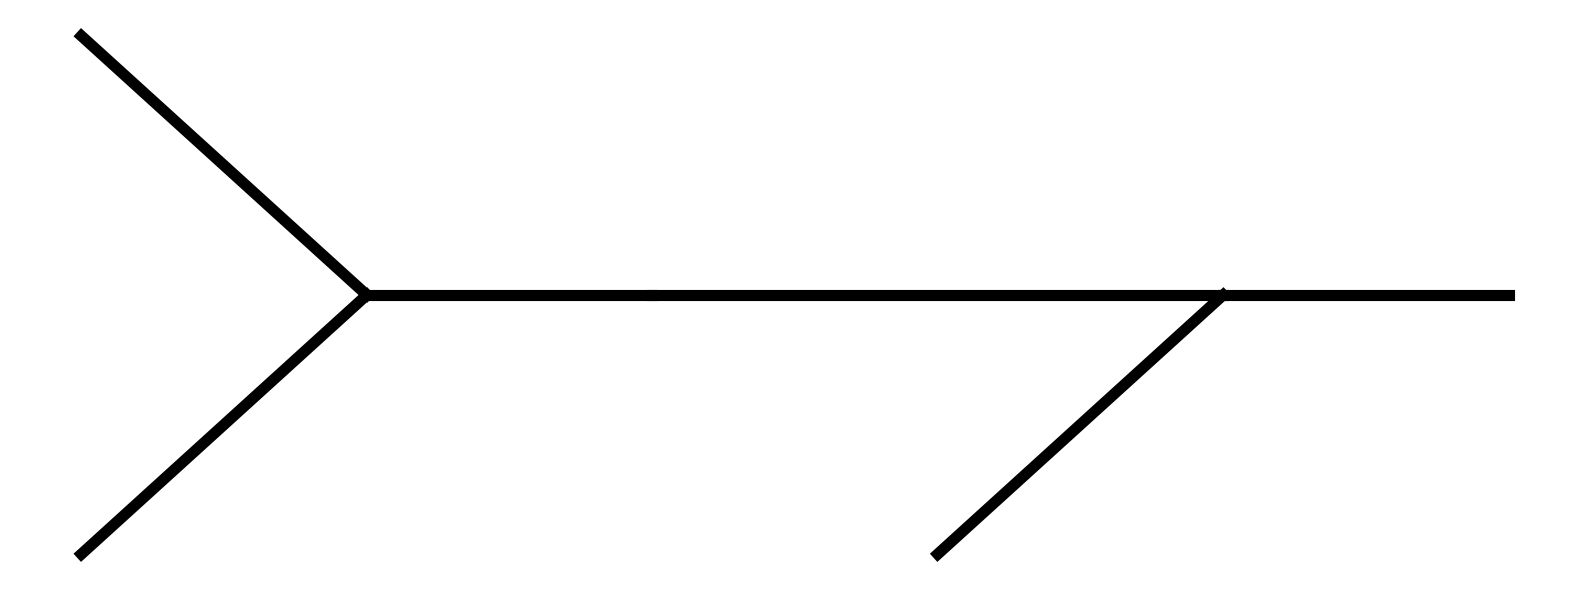
\includegraphics[width=\textwidth]{plots/1to3.png}
    \end{subfigure}%
\end{figure*}

Similar procedure is followed for both the second and fourth terms, producing similar results.
It is in the third term where more possibilities arise, since now either one 
connection or two connections can be considered, producing 2 different diagrams, of multiplicity 2.

\begin{figure*}[h!]
  \centering
  % switch into math mode, start a stretchy left parenthesis 
    % first subfigure
    \begin{subfigure}[t]{.1\textwidth}
    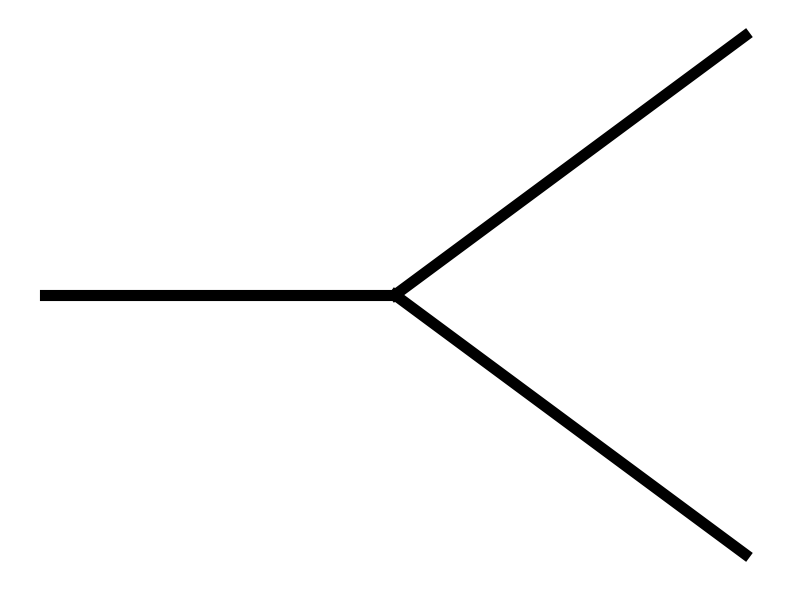
\includegraphics[width=\textwidth]{plots/2to1.png}
    \end{subfigure}%
    \begin{subfigure}[t]{.1\textwidth}
    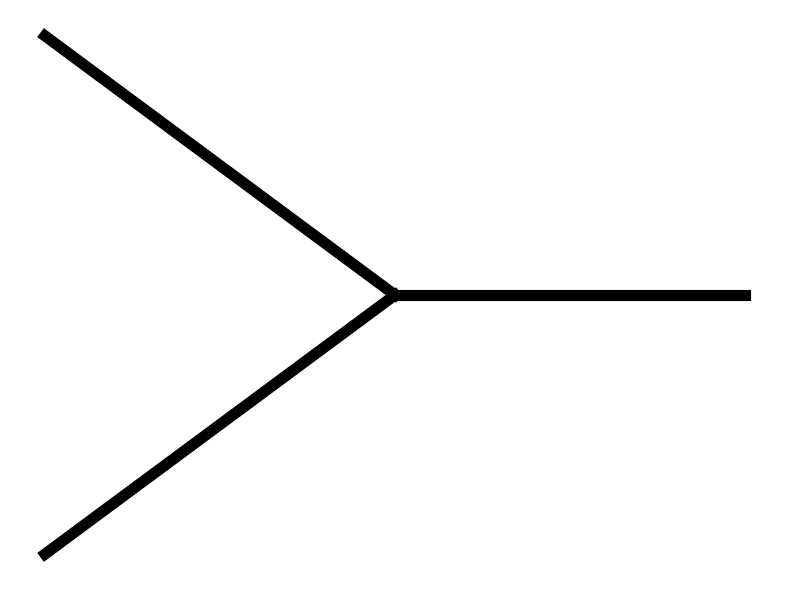
\includegraphics[width=\textwidth]{plots/1to2.png}
    \end{subfigure}%
    $\displaystyle \quad % space between
    \raisebox{1.8\height}{\LARGE $\to$} $
    $\displaystyle \quad % space between
    \raisebox{1.2\height}{\Large $2\cdot$} $
    \begin{subfigure}[t]{.2\textwidth}
    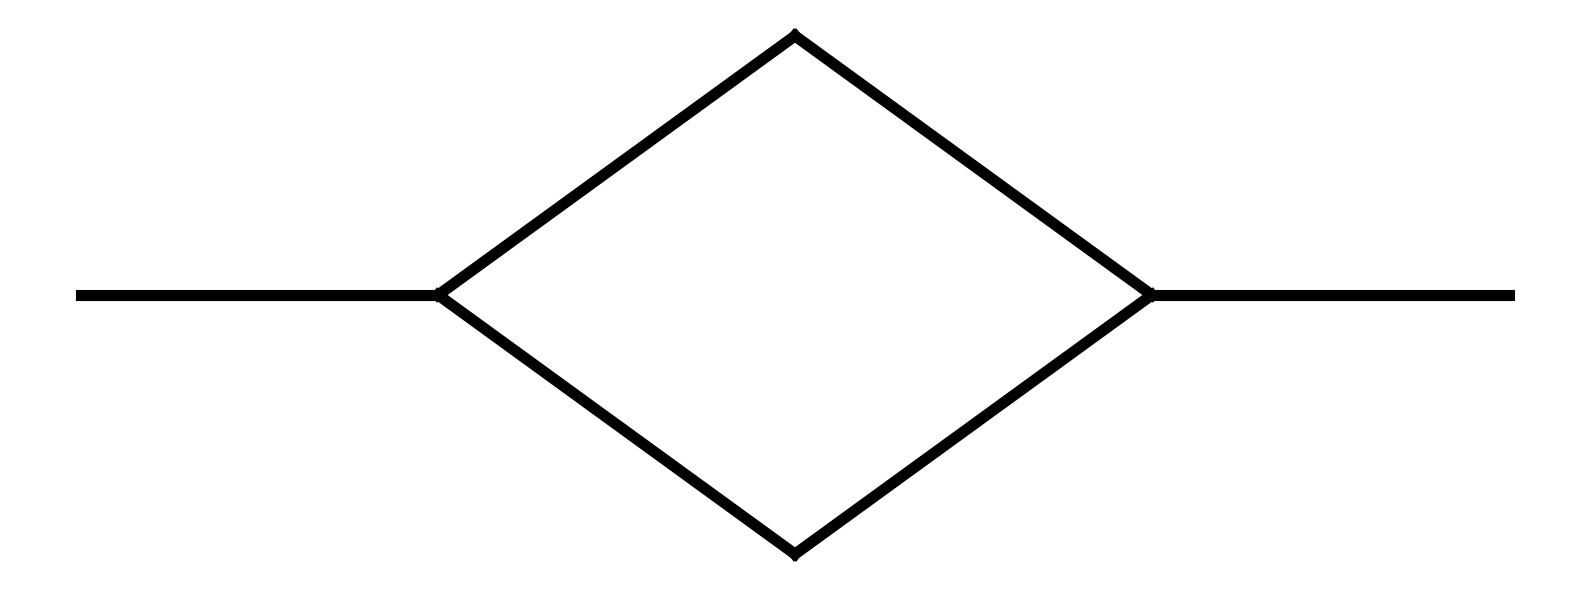
\includegraphics[width=\textwidth]{plots/1to1_1.png}
    \end{subfigure}%
    \raisebox{1.3\height}{\Large $+$}\quad
    \raisebox{1.2\height}{\Large $4\cdot$}
    \begin{subfigure}[t]{.2\textwidth}
    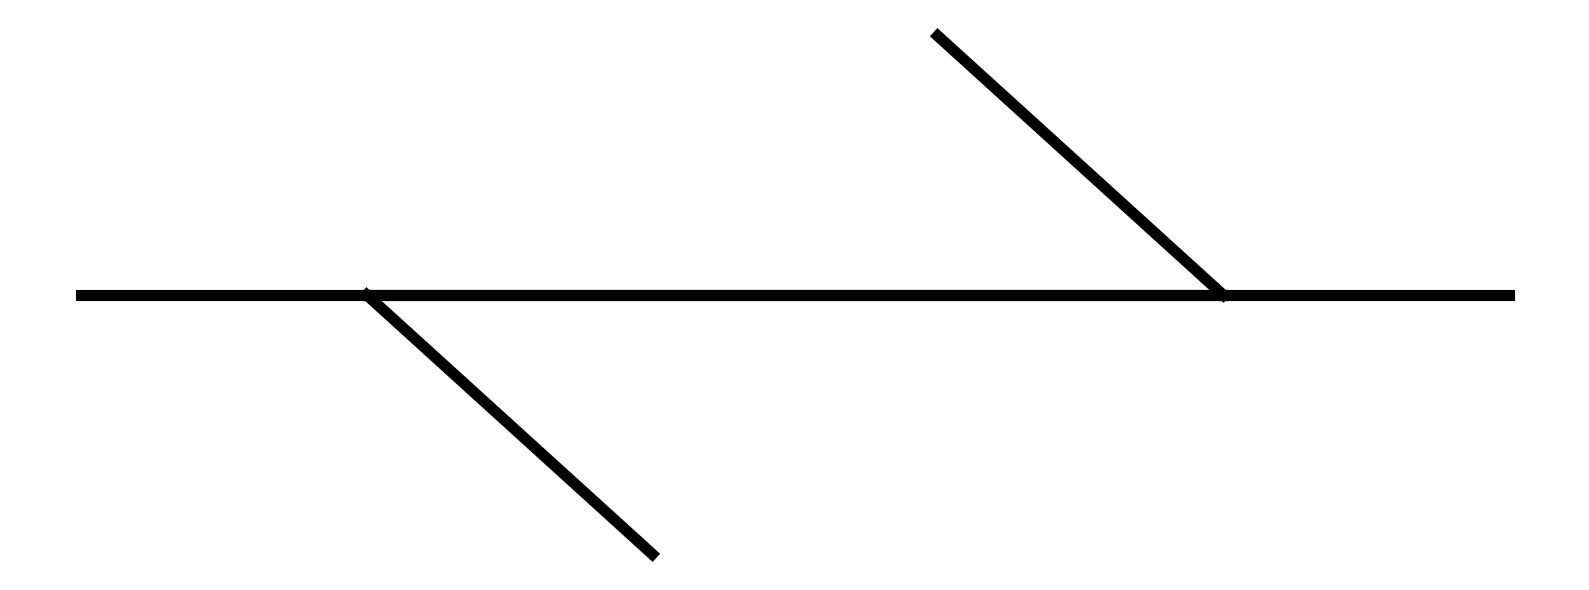
\includegraphics[width=\textwidth]{plots/1to1_2.png}
    \end{subfigure}%
\end{figure*}

The first diagram will produce a loop, and thus a counterterm will be added to the
list of diagram, to cancel the divergence produced.

\subsection{Applied to gluon interactions} \label{sec:applied_gluons}
Although the focus of this thesis is only gluons, 
the program can be adapted to consider new types of particles.

The instantaneous 
process considered as a new type of particle, need to respect the time 
evolution of the system, meaning that in the eyes of the program, since the x-coordinate
is different, the 
instantaneous interaction is no longer considered to be instantaneous, 
but rather a process that
happens in a certain time interval. But since the instantaneous interactions 
really encodes a vertex, no other vertices can be present during the instantaneous
interaction, and the program will ensure that this is the case.

\newpage

\section{Diagrams obtained} \label{sec:diagrams}

In this section, we will present the diagrams obtained from the program. At 
each order, we will consider the most relevant types of interaction.

\subsection{Order 2}
The second order diagrams correspond to the canonical diagrams of order 2,
plus the diagrams obtained from the combination of the canonical diagrams of order 1 with 
itself and counterterms, shown in figure \ref{fig:order2_from_order1}.

\begin{figure*}[h!]
    \centering
    \begin{subfigure}[t]{0.24\textwidth}
        \centering
        \includegraphics[width=\textwidth]{plots/order2/from_order1/1.png}
        \caption{ }
        \label{fig:order2_from_order1/1}
    \end{subfigure}%
    \hfill
    \begin{subfigure}[t]{0.24\textwidth}
        \centering
        \includegraphics[width=\textwidth]{plots/order2/from_order1/2.png}
        \caption{ }
        \label{fig:order2_from_order1/2}
    \end{subfigure}
    \hfill
    \begin{subfigure}[t]{0.24\textwidth}
        \centering
        \includegraphics[width=\textwidth]{plots/order2/from_order1/3.png}
        \caption{ }
        \label{fig:order2_from_order1/3}
    \end{subfigure}
    \hfill
    \begin{subfigure}[t]{0.24\textwidth}
        \centering
        \includegraphics[width=\textwidth]{plots/order2/from_order1/4.png}
        \caption{ }
        \label{fig:order2_from_order1/4}
    \end{subfigure}
    \hfill
    \begin{subfigure}[t]{0.24\textwidth}
        \centering
        \includegraphics[width=\textwidth]{plots/order2/from_order1/5.png}
        \caption{ }
        \label{fig:order2_from_order1/5}
    \end{subfigure}
    \begin{subfigure}[t]{0.24\textwidth}
        \centering
        \includegraphics[width=\textwidth]{plots/order2/from_order1/counterterms/1.png}
        \caption{ }
        \label{fig:order2_from_order1/counterterms}
    \end{subfigure}
    \caption{Some examples of diagrams of second order, obtained from the combination of the canonical
diagrams of order 1. Fig. (f) represents second-order
counterterm.}
    \label{fig:order2_from_order1}
\end{figure*}

The diagram \ref{fig:order2_from_order1/1} is the combination of 2 
\ref{fig:cannonical1_1} diagrams, where one of the outgoing gluon from the first
diagram becomes the incoming gluon of the second diagram. 

\begin{figure*}[h!]
  \centering
  % switch into math mode, start a stretchy left parenthesis
  $\displaystyle
      % now vcenter the whole block so its height is taken into account
      \vcenter{%
        \hbox{%  
          % first subfigure
          \begin{subfigure}[t]{.15\textwidth}
            \includegraphics[width=\textwidth]{plots/1to2.png}
          \end{subfigure}%
          
          % second subfigure
          \begin{subfigure}[t]{.15\textwidth}
            \includegraphics[width=\textwidth]{plots/1to2.png}
          \end{subfigure}%
        \quad % space between
          \raisebox{3\height}{\LARGE $\to$}\quad
        \raisebox{-0.1\height}{%  % lower it by 20% of its own height
        \begin{subfigure}[t]{0.3\textwidth}
          \centering
          \includegraphics[width=\textwidth]{plots/order2/from_order1/1.png}
        \end{subfigure}%
      }%
        }% end \hbox
        }% end \vcenter
    $ 
\end{figure*}

Similarly, the diagram
\ref{fig:order2_from_order1/5} is the combination of 2 \ref{fig:cannonical1_2} diagrams, 
the outgoing gluon of the first diagram is the one of the incoming gluon to the 
second diagram.

\begin{figure*}[h!]
  \centering
  % switch into math mode, start a stretchy left parenthesis
  $\displaystyle
      % now vcenter the whole block so its height is taken into account
      \vcenter{%
        \hbox{%  
          % first subfigure
          \begin{subfigure}[t]{.15\textwidth}
            \includegraphics[width=\textwidth]{plots/1to2.png}
          \end{subfigure}%
          
          % second subfigure
          \begin{subfigure}[t]{.15\textwidth}
            \includegraphics[width=\textwidth]{plots/2to1.png}
          \end{subfigure}%
        \quad % space between
          \raisebox{3\height}{\LARGE $\to$}\quad
        \raisebox{-0.1\height}{%  % lower it by 20% of its own height
        \begin{subfigure}[t]{0.3\textwidth}
          \centering
          \includegraphics[width=\textwidth]{plots/order2/from_order1/4.png}
        \end{subfigure}%
      }%
        }% end \hbox
        }% end \vcenter
    $ 
\end{figure*}

\newpage

As for the diagrams \ref{fig:order2_from_order1/2} and \ref{fig:order2_from_order1/3}, 
both result from the combination of \ref{fig:cannonical1_1} and \ref{fig:cannonical1_2} diagrams,
in that order, where the different diagrams are obtained depending on the number of
connections between the incoming and outgoing gluons.
~
\begin{figure*}[h!]
  \centering
  % switch into math mode, start a stretchy left parenthesis
  $\displaystyle
      % now vcenter the whole block so its height is taken into account
      \vcenter{%
        \hbox{%  
          % first subfigure
          \begin{subfigure}[t]{.13\textwidth}
            \includegraphics[width=\textwidth]{plots/2to1.png}
          \end{subfigure}%
          
          % second subfigure
          \begin{subfigure}[t]{.13\textwidth}
            \includegraphics[width=\textwidth]{plots/1to2.png}
          \end{subfigure}%
        \quad % space between
          \raisebox{2.5\height}{\LARGE $\to$}\quad
        \raisebox{-0.2\height}{%  % lower it by 20% of its own height
        \begin{subfigure}[t]{0.25\textwidth}
          \centering
          \includegraphics[width=\textwidth]{plots/order2/from_order1/2.png}
        \end{subfigure}%
      }% 
      \raisebox{1.5\height}{\LARGE $+$}
      \raisebox{1.5\height}{\Large $h.c.$}
      
        \raisebox{1.5\height}{\LARGE $+$}\quad
        \raisebox{-0.2\height}{%  % lower it by 20% of its own height
        \begin{subfigure}[t]{0.25\textwidth}
          \centering
          \includegraphics[width=\textwidth]{plots/order2/from_order1/3.png}
        \end{subfigure}%
      }%
        }% end \hbox
        }% end \vcenter
    $ 
\end{figure*}


The diagram \ref{fig:order2_from_order1/4} is the combination of the
\ref{fig:cannonical1_2} and \ref{fig:cannonical1_1} diagrams, where the outgoing gluon
of the first diagram is the incoming gluon of the second diagram.

\begin{figure*}[h!]
  \centering
  % switch into math mode, start a stretchy left parenthesis
  $\displaystyle
      % now vcenter the whole block so its height is taken into account
      \vcenter{%
        \hbox{%  
          % first subfigure
          \begin{subfigure}[t]{.15\textwidth}
            \includegraphics[width=\textwidth]{plots/2to1.png}
          \end{subfigure}%
          
          % second subfigure
          \begin{subfigure}[t]{.15\textwidth}
            \includegraphics[width=\textwidth]{plots/2to1.png}
          \end{subfigure}%
        \quad % space between
          \raisebox{3\height}{\LARGE $\to$}\quad
        \raisebox{-0.1\height}{%  % lower it by 20% of its own height
        \begin{subfigure}[t]{0.3\textwidth}
          \centering
          \includegraphics[width=\textwidth]{plots/order2/from_order1/5.png}
        \end{subfigure}%
      }%
        }% end \hbox
        }% end \vcenter
    $ 
\end{figure*}

Finally, the diagram \ref{fig:order2_from_order1/counterterms} is the counterterm
associated with the second order diagrams, canceling the divergences that arises.

\subsection{Three gluon vertex: 1 gluon to 2 gluons}

Considering the process of 1 gluon going to 2 gluons, up till 
order 3, the diagrams obtained from the program are shown in the figures 
\ref{fig:order3_1to2} and \ref{fig:order3_1to2/counterterms}.

\begin{figure*}[h!]
    \centering
    \begin{subfigure}[t]{0.24\textwidth}
        \centering
        \includegraphics[width=\textwidth]{plots/order3/order3_1to2/1.png}
        \caption{ }
    \end{subfigure}%
    \hfill
    \begin{subfigure}[t]{0.24\textwidth}
        \centering
        \includegraphics[width=\textwidth]{plots/order3/order3_1to2/2.png}
        \caption{ }
    \end{subfigure}
    \hfill
    \begin{subfigure}[t]{0.24\textwidth}
        \centering
        \includegraphics[width=\textwidth]{plots/order3/order3_1to2/3.png}
        \caption{ }
    \end{subfigure}
    \hfill
    \begin{subfigure}[t]{0.24\textwidth}
        \centering
        \includegraphics[width=\textwidth]{plots/order3/order3_1to2/4.png}
        \caption{ }
    \end{subfigure}
    \hfill
    \begin{subfigure}[t]{0.24\textwidth}
        \centering
        \includegraphics[width=\textwidth]{plots/order3/order3_1to2/5.png}
        \caption{ }
        \label{fig:order3_1to2/5}
    \end{subfigure}
    \hfill  
    \begin{subfigure}[t]{0.24\textwidth}
        \centering
        \includegraphics[width=\textwidth]{plots/order3/order3_1to2/6.png}
        \caption{ }
        \label{fig:order3_1to2/6}
    \end{subfigure}
    \hfill
    \begin{subfigure}[t]{0.24\textwidth}
        \centering
        \includegraphics[width=\textwidth]{plots/order3/order3_1to2/7.png}
        \caption{ }
    \end{subfigure}
    \hfill 
    \begin{subfigure}[t]{0.24\textwidth}
        \centering
        \includegraphics[width=\textwidth]{plots/order3/order3_1to2/8.png}
        \caption{ }
    \end{subfigure}
    \caption{Diagrams of third order, contributing to the three-gluon vertex.}
    \label{fig:order3_1to2}
\end{figure*}

\begin{figure*}[h!]
    \centering
    \begin{subfigure}[t]{0.24\textwidth}
        \centering
        \includegraphics[width=\textwidth]{plots/order3/order3_1to2/counterterms/2.png}
        \caption{ }
    \end{subfigure}
    \hfill
    \begin{subfigure}[t]{0.24\textwidth}
        \centering
        \includegraphics[width=\textwidth]{plots/order3/order3_1to2/counterterms/3.png}
        \caption{ }
    \end{subfigure}
    \hfill
    \begin{subfigure}[t]{0.24\textwidth}
        \centering
        \includegraphics[width=\textwidth]{plots/order3/order3_1to2/counterterms/4.png}
        \caption{ }
        \label{fig:order3_1to2/counterterms/4}
    \end{subfigure}
    \hfill
    \begin{subfigure}[t]{0.24\textwidth}
        \centering
        \includegraphics[width=\textwidth]{plots/order3/order3_1to2/counterterms/5.png}
        \caption{ }
        \label{fig:order3_1to2/counterterms/5}
    \end{subfigure}
    \hfill
    \centering
    \begin{subfigure}[t]{0.24\textwidth}
        \centering
        \includegraphics[width=\textwidth]{plots/order3/order3_1to2/counterterms/1.png}
        \caption{ }
    \end{subfigure}%
    \caption{Third-order contributions containing counterterms [graphs (a) to (d)] and the third order
    counterterm [graph (e)].}
    \label{fig:order3_1to2/counterterms}
\end{figure*}

Depending on the types of particles in the process, we can deduce the origin of the 
different diagrams. Since the dotted lines are only present in the canonical diagrams 
of order 2.

\newpage

Referring to the problems mentioned in Section \ref{sec:applied_gluons}, the diagrams 
with dotted lines are instantaneous interactions, but the program considers them
as a new type of particle, there are some artifacts that arise from this
approach. For instance, the diagrams \ref{fig:order3_1to2/5} and \ref{fig:order3_1to2/6} are actually the same 
diagram, due to instant process being instantaneous. For any other particle, these 
2 diagrams would be different, due to the importance of the order in the interactions.
Hence, the program keeps them different, to avoid the loss of generality.

Comparing with the 3rd order contribution diagrams in \cite{QCDG}, the same diagrams
for the three-gluon vertex are obtained, proving the validity of the program to reproduce the same results.

\subsection{Self-energy: Gluon's effective mass}

The self-energy describes the interaction of a gluon with itself, leading to 
modifications of the propagator and the effective mass of the gluon, such that 
at the infrared limit, the gluon mimics a massive particle.
This is also reflected in or Hamiltonian formalism.

Each order of the effective Hamiltonian contains parts that contribute to different 
types of interactions, 

\begin{equation}
    \mathcal{H}_{n t} = \mathcal{H}_{n t}^{(1 \rightarrow 1)} + \mathcal{H}_{n t}^{(1 \rightarrow 2)} + 
    \mathcal{H}_{n t}^{(2 \rightarrow 1)} + \ldots
\end{equation}
where $\mathcal{H}_{n t}^{(1 \rightarrow 1)}$ is the part of the Hamiltonian that
contributes to the process of 1 gluon going to 1 gluon, $\mathcal{H}_{n t}^{(1 \rightarrow 2)}$ 
is the part that contributes to the process of 1 gluon going to 2 gluons, and so on.

This effective Hamiltonian can be expressed in terms of creation and annihilation operators,
similar to Eqs.\eqref{eq:H_A^2}, as follows,

\begin{equation}
    \mathcal{H}_{n t}^{(1 \rightarrow 1)} = \int [k] g^n \Sigma_t^{(n)} (k) 
    a^{\dagger}_t (k) a_t (k),
    \label{eq:H_1to1}
\end{equation}
where $\Sigma_t^{(n)} (k)$ is the self-energy correction at order $n$ for the gluon
self-energy. Comparing with the expression for the kinetic energy of the gluon, Eq.
\eqref{eq:H_1to1} introduces a correction, obtaining an effective kinetic energy, where
$\Sigma_t^{(n)} (k)$ is interpreted as a mass-like term,

\begin{equation}
    m_{n t}^2 (k) = g^n \Sigma_t^{(n)} (k).
\end{equation}

This way to study the self-energy of the gluon, we need to focus on the part of the
Hamiltonian that contributes to the process of 1 gluon going to 1 gluon,
\begin{equation}
    \mathcal{H}_{t}^{(1 \rightarrow 1)} = \mathcal{H}_{2 t}^{(1 \rightarrow 1)} + 
    \mathcal{H}_{4 t}^{(1 \rightarrow 1)} + \ldots
\end{equation}

As for the effective kinetic term of the gluon, it verifies,

\begin{equation}
    k_{eff}^- = \frac{k^{\perp 2} + m_{t}^2 (k)}{k^+}, 
\end{equation}
with $m_{t}^2 (k)$ being the effective mass considering all contributions from the 
expansion,

\begin{equation}
    m_{t}^2 (k) = g^2 \Sigma_t^{(2)} (k) + g^4 \Sigma_t^{(4)} (k) + g^6 \Sigma_t^{(6)} (k) + \ldots
\end{equation} 

\begin{comment}

This way the gauge boson propagator in momentum space is of the form, 

\begin{equation}
    D(p^2) \sim \frac{1}{p^2 - m_{t}^2} 
\end{equation}
where $m_{t}$ is the effective mass of the gluon at a particular scale, arising due 
to the presence of loop corrections. 

To obtain the effective mass of the gluon, we need to consider one to one gluon interactions,
or equivalently the propagation of a gluon. This way the effective mass can be obtained 
by considering the sum on the contributions of the diagrams at each order,

\begin{equation}
    m_{t}^2 = g^2 m^2_{(2), t} + g^4 m^2_{(4), t} + g^6 m^2_{(6), t} + \ldots
\end{equation}
with $m^2_{(n), t}$ being the effective mass correction at order $n$.

\end{comment}

Then, it is in our best interest to obtain all the diagrams at each order that contribute
to the gluon's self-energy.

At order 2, the diagram that contributes to the gluon's self-energy is presented in figure 
\ref{fig:order2_from_order1/3}  and \ref{fig:order2_from_order1/counterterms}.
At order 4, the diagrams that contribute to the gluon's self-energy are shown in figure
\ref{fig:order4_1to1}.

\begin{figure*}[h!]
    \centering
    \begin{subfigure}[t]{0.19\textwidth}
        \centering
        \includegraphics[width=\textwidth]{plots/order4_1to1/1.png}
        \caption{ }
    \end{subfigure}%
    \begin{subfigure}[t]{0.19\textwidth}
        \centering
        \includegraphics[width=\textwidth]{plots/order4_1to1/2.png}
        \caption{ }
    \end{subfigure}
    \begin{subfigure}[t]{0.19\textwidth}
        \centering
        \includegraphics[width=\textwidth]{plots/order4_1to1/3.png}
        \caption{ }
    \end{subfigure}
    \begin{subfigure}[t]{0.19\textwidth}
        \centering
        \includegraphics[width=\textwidth]{plots/order4_1to1/4.png}
        \caption{ }
    \end{subfigure}
    \begin{subfigure}[t]{0.19\textwidth}
        \centering
        \includegraphics[width=\textwidth]{plots/order4_1to1/5.png}
        \caption{ }
    \end{subfigure}
    \begin{subfigure}[t]{0.19\textwidth}
        \centering
        \includegraphics[width=\textwidth]{plots/order4_1to1/6.png}
        \caption{ }
    \end{subfigure}
    \begin{subfigure}[t]{0.19\textwidth}
        \centering
        \includegraphics[width=\textwidth]{plots/order4_1to1/7.png}
        \caption{ }
    \end{subfigure}
    \begin{subfigure}[t]{0.19\textwidth}
        \centering
        \includegraphics[width=\textwidth]{plots/order4_1to1/counterterms/1.png}
        \caption{ }
    \end{subfigure}
    \begin{subfigure}[t]{0.19\textwidth}
        \centering
        \includegraphics[width=\textwidth]{plots/order4_1to1/counterterms/3.png}
        \caption{ }
        
    \end{subfigure}
    \begin{subfigure}[t]{0.19\textwidth}
        \centering
        \includegraphics[width=\textwidth]{plots/order4_1to1/counterterms/4.png}
        \caption{ }
        
    \end{subfigure}
    \begin{subfigure}[t]{0.19\textwidth}
        \centering
        \includegraphics[width=\textwidth]{plots/order4_1to1/counterterms/5.png}
        \caption{ }
        
    \end{subfigure}
    \begin{subfigure}[t]{0.19\textwidth}
        \centering
        \includegraphics[width=\textwidth]{plots/order4_1to1/counterterms/6.png}
        \caption{ }
        
    \end{subfigure}

    \caption{Diagrams of fourth order, contributing to the gluon's self-energy,
    with (h)-(k) diagrams with counterterms of order 2, and (l) the counterterm 
    of order 4.}
    \label{fig:order4_1to1}
    
\end{figure*}

This thesis focuses on the generation of the diagrams, and thus we will not
consider any calculation beyond this analysis, since
they are far from the scope of this work. However, these posses a visual 
starting point for future calculations.

\begin{comment}

\subsubsection{Additional implications: Quark interactions}
The implication of the gluon's self-energy extend to the quark interactions, since the gluon
is the mediator of the strong force, and thus the effective mass of the gluon will 
impact the results of the quark interactions.

\begin{figure} [h!]
    \centering
    \includegraphics[width=0.5\textwidth]{plots/qq_int.jpg}
    \caption{Quark-quark interaction, mediated by gluons with an effective mass. The quarks
    are represented by the solid lines, while the gluons are represented by the wavy lines.
    The big dot in the middle represents the effective mass of the gluon.}

    \label{fig:qq_int}
\end{figure}

In the case of massless propagators, the interactions between 
particles are long-range, while for massive propagators, the interactions are short-range.
Meaning that the effective mass of the gluon will screen the color interactions at
large distances, modifying the potential between quarks in the infrared regime.

\end{comment}

\newpage

\subsection{Bound states: Glueballs}

Glueballs are color-singlet bound states of 2 or more interacting gluons, unlike mesons
and baryons, which involve quarks and antiquarks, glueballs are composed solely of gluons.
The existence of glueballs is predicted as a consequence of the non-abelian nature of QCD, where gluons
interact strongly enough with each other to become dynamically confined. However,
they are not confirmed experimentally nowadays. A deep theoretical understanding of 
their dynamic structure is welcomed.

The two to two gluon interaction is the simplest case of a glueball, and it can be
obtained from the program by considering the process of 2 gluons going to 2 gluons.
The diagrams obtained from the program are shown in figure \ref{fig:order4_2to2}.

\begin{figure*}[h!]
    \centering
    \begin{subfigure}[t]{0.16\textwidth}
        \centering
        \includegraphics[width=\textwidth]{plots/order4_2to2/1.png}
    \end{subfigure}%
    \hfill
    \begin{subfigure}[t]{0.16\textwidth}
        \centering
        \includegraphics[width=\textwidth]{plots/order4_2to2/2.png}
    \end{subfigure}
    \hfill
    \begin{subfigure}[t]{0.16\textwidth}
        \centering
        \includegraphics[width=\textwidth]{plots/order4_2to2/3.png}
    \end{subfigure}
    \hfill
    \begin{subfigure}[t]{0.16\textwidth}
        \centering
        \includegraphics[width=\textwidth]{plots/order4_2to2/4.png}
    \end{subfigure}
    \hfill
    \begin{subfigure}[t]{0.16\textwidth}
        \centering
        \includegraphics[width=\textwidth]{plots/order4_2to2/5.png}
    \end{subfigure}
    \hfill
    \begin{subfigure}[t]{0.16\textwidth}
        \centering
        \includegraphics[width=\textwidth]{plots/order4_2to2/6.png}
    \end{subfigure}
    \hfill
    \begin{subfigure}[t]{0.16\textwidth}
        \centering
        \includegraphics[width=\textwidth]{plots/order4_2to2/7.png}
    \end{subfigure}
    \hfill
    \begin{subfigure}[t]{0.16\textwidth}
        \centering
        \includegraphics[width=\textwidth]{plots/order4_2to2/8.png}
    \end{subfigure}
    \hfill 
    \begin{subfigure}[t]{0.16\textwidth}
        \centering
        \includegraphics[width=\textwidth]{plots/order4_2to2/9.png}
    \end{subfigure}
    \hfill
    \begin{subfigure}[t]{0.16\textwidth}
        \centering
        \includegraphics[width=\textwidth]{plots/order4_2to2/10.png}
    \end{subfigure}
    \hfill 
    \begin{subfigure}[t]{0.16\textwidth}
        \centering
        \includegraphics[width=\textwidth]{plots/order4_2to2/11.png}
    \end{subfigure}
    \hfill
    \begin{subfigure}[t]{0.16\textwidth}
        \centering
        \includegraphics[width=\textwidth]{plots/order4_2to2/12.png}
    \end{subfigure}
    \hfill
    \begin{subfigure}[t]{0.16\textwidth}
        \centering
        \includegraphics[width=\textwidth]{plots/order4_2to2/13.png}
    \end{subfigure}
    \hfill
    \begin{subfigure}[t]{0.16\textwidth}
        \centering
        \includegraphics[width=\textwidth]{plots/order4_2to2/14.png}
    \end{subfigure}
    \hfill
    \begin{subfigure}[t]{0.16\textwidth}
        \centering
        \includegraphics[width=\textwidth]{plots/order4_2to2/15.png}
    \end{subfigure}
    \hfill
    \begin{subfigure}[t]{0.16\textwidth}
        \centering
        \includegraphics[width=\textwidth]{plots/order4_2to2/16.png}
    \end{subfigure}
    \hfill
    \begin{subfigure}[t]{0.16\textwidth}
        \centering
        \includegraphics[width=\textwidth]{plots/order4_2to2/17.png}
    \end{subfigure}
    \hfill
    \begin{subfigure}[t]{0.16\textwidth}
        \centering
        \includegraphics[width=\textwidth]{plots/order4_2to2/18.png}
    \end{subfigure}
    \hfill
    \begin{subfigure}[t]{0.16\textwidth}
        \centering
        \includegraphics[width=\textwidth]{plots/order4_2to2/19.png}
    \end{subfigure}
    \hfill
    \begin{subfigure}[t]{0.16\textwidth}
        \centering
        \includegraphics[width=\textwidth]{plots/order4_2to2/20.png}
    \end{subfigure}
    \hfill
    \begin{subfigure}[t]{0.16\textwidth}
        \centering
        \includegraphics[width=\textwidth]{plots/order4_2to2/21.png}
    \end{subfigure}
    \hfill
    \begin{subfigure}[t]{0.16\textwidth}
        \centering
        \includegraphics[width=\textwidth]{plots/order4_2to2/22.png}
    \end{subfigure}
    \hfill
    \begin{subfigure}[t]{0.16\textwidth}
        \centering
        \includegraphics[width=\textwidth]{plots/order4_2to2/23.png}
    \end{subfigure}
    \hfill
    \begin{subfigure}[t]{0.16\textwidth}
        \centering
        \includegraphics[width=\textwidth]{plots/order4_2to2/24.png}
    \end{subfigure}
    \hfill
    \begin{subfigure}[t]{0.16\textwidth}
        \centering
        \includegraphics[width=\textwidth]{plots/order4_2to2/25.png}
    \end{subfigure}
    \hfill
    \begin{subfigure}[t]{0.16\textwidth}
        \centering
        \includegraphics[width=\textwidth]{plots/order4_2to2/26.png}
    \end{subfigure}
    \hfill
    \begin{subfigure}[t]{0.16\textwidth}
        \centering
        \includegraphics[width=\textwidth]{plots/order4_2to2/27.png}
    \end{subfigure}
    \hfill
    \begin{subfigure}[t]{0.16\textwidth}
        \centering
        \includegraphics[width=\textwidth]{plots/order4_2to2/28.png}
    \end{subfigure}
    \hfill
    \begin{subfigure}[t]{0.16\textwidth}
        \centering
        \includegraphics[width=\textwidth]{plots/order4_2to2/29.png}
    \end{subfigure}
    \hfill
    \begin{subfigure}[t]{0.16\textwidth}
        \centering
        \includegraphics[width=\textwidth]{plots/order4_2to2/30.png}
    \end{subfigure}
    \hfill
    \begin{subfigure}[t]{0.16\textwidth}
        \centering
        \includegraphics[width=\textwidth]{plots/order4_2to2/31.png}
    \end{subfigure}
    \hfill
    \begin{subfigure}[t]{0.16\textwidth}
        \centering
        \includegraphics[width=\textwidth]{plots/order4_2to2/32.png}
    \end{subfigure}
    \hfill
    \begin{subfigure}[t]{0.16\textwidth}
        \centering
        \includegraphics[width=\textwidth]{plots/order4_2to2/33.png}
    \end{subfigure}
    \hfill
    \begin{subfigure}[t]{0.16\textwidth}
        \centering
        \includegraphics[width=\textwidth]{plots/order4_2to2/34.png}
    \end{subfigure}
    \hfill
    \begin{subfigure}[t]{0.16\textwidth}
        \centering
        \includegraphics[width=\textwidth]{plots/order4_2to2/35.png}
    \end{subfigure}
    \hfill
    \begin{subfigure}[t]{0.16\textwidth}
        \centering
        \includegraphics[width=\textwidth]{plots/order4_2to2/36.png}
    \end{subfigure}


    \begin{subfigure}[t]{0.1\textwidth}
        \centering
        {\LARGE $\ldots$}
    \end{subfigure}
    \vspace{0.5cm}

    \begin{subfigure}[t]{0.16\textwidth}
        \centering
        \includegraphics[width=\textwidth]{plots/order4_2to2/counterterms/1.png}
    \end{subfigure}%
    \hfill
    \begin{subfigure}[t]{0.16\textwidth}
        \centering
        \includegraphics[width=\textwidth]{plots/order4_2to2/counterterms/2.png}
    \end{subfigure}
    \hfill
    \begin{subfigure}[t]{0.16\textwidth}
        \centering
        \includegraphics[width=\textwidth]{plots/order4_2to2/counterterms/3.png}
    \end{subfigure}
    \hfill
    \begin{subfigure}[t]{0.16\textwidth}
        \centering
        \includegraphics[width=\textwidth]{plots/order4_2to2/counterterms/4.png}
    \end{subfigure}
    \hfill
    \begin{subfigure}[t]{0.16\textwidth}
        \centering
        \includegraphics[width=\textwidth]{plots/order4_2to2/counterterms/5.png}
    \end{subfigure}
    \hfill
    \begin{subfigure}[t]{0.16\textwidth}
        \centering
        \includegraphics[width=\textwidth]{plots/order4_2to2/counterterms/6.png}
    \end{subfigure}
    \hfill
    \begin{subfigure}[t]{0.16\textwidth}
        \centering
        \includegraphics[width=\textwidth]{plots/order4_2to2/counterterms/7.png}
    \end{subfigure}
    \hfill
    \begin{subfigure}[t]{0.16\textwidth}
        \centering
        \includegraphics[width=\textwidth]{plots/order4_2to2/counterterms/8.png}
    \end{subfigure}
    \hfill 
    \begin{subfigure}[t]{0.16\textwidth}
        \centering
        \includegraphics[width=\textwidth]{plots/order4_2to2/counterterms/9.png}
    \end{subfigure}
    \hfill
    \begin{subfigure}[t]{0.16\textwidth}
        \centering
        \includegraphics[width=\textwidth]{plots/order4_2to2/counterterms/10.png}
    \end{subfigure}
    \hfill
    \begin{subfigure}[t]{0.16\textwidth}
        \centering
        \includegraphics[width=\textwidth]{plots/order4_2to2/counterterms/11.png}
    \end{subfigure}
    \hfill
    \begin{subfigure}[t]{0.16\textwidth}
        \centering
        \includegraphics[width=\textwidth]{plots/order4_2to2/counterterms/12.png}
    \end{subfigure}
    \hfill
    \begin{subfigure}[t]{0.16\textwidth}
        \centering
        \includegraphics[width=\textwidth]{plots/order4_2to2/counterterms/13.png}
    \end{subfigure}
    \hfill
    \begin{subfigure}[t]{0.16\textwidth}
        \centering
        \includegraphics[width=\textwidth]{plots/order4_2to2/counterterms/14.png}
    \end{subfigure}
    \hfill
    \begin{subfigure}[t]{0.16\textwidth}
        \centering
        \includegraphics[width=\textwidth]{plots/order4_2to2/counterterms/15.png}
    \end{subfigure}
    \hfill
    \begin{subfigure}[t]{0.16\textwidth}
        \centering
        \includegraphics[width=\textwidth]{plots/order4_2to2/counterterms/16.png}
    \end{subfigure}
    \hfill
    \begin{subfigure}[t]{0.16\textwidth}
        \centering
        \includegraphics[width=\textwidth]{plots/order4_2to2/counterterms/17.png}
    \end{subfigure}
    \hfill  
    \begin{subfigure}[t]{0.16\textwidth}
        \centering
        \includegraphics[width=\textwidth]{plots/order4_2to2/counterterms/18.png}
    \end{subfigure}
    \hfill
    \begin{subfigure}[t]{0.1\textwidth}
        \centering
        {\LARGE $\ldots$}
    \end{subfigure}
    \hfill
    \caption{Some diagrams of fourth order, contributing to the process of 
    2 gluons going to 2 gluons.}
    \label{fig:order4_2to2}
\end{figure*}

\begin{figure*}[h!]
    \centering
    \begin{subfigure}[t]{0.16\textwidth}
        \centering
        \includegraphics[width=\textwidth]{plots/order6_2to2/1.png}
    \end{subfigure}%
    \hfill
    \begin{subfigure}[t]{0.16\textwidth}
        \centering
        \includegraphics[width=\textwidth]{plots/order6_2to2/2.png}
    \end{subfigure}
    \hfill
    \begin{subfigure}[t]{0.16\textwidth}
        \centering
        \includegraphics[width=\textwidth]{plots/order6_2to2/3.png}
    \end{subfigure}
    \hfill
    \begin{subfigure}[t]{0.16\textwidth}
        \centering
        \includegraphics[width=\textwidth]{plots/order6_2to2/4.png}
    \end{subfigure}
    \hfill
    \begin{subfigure}[t]{0.16\textwidth}
        \centering
        \includegraphics[width=\textwidth]{plots/order6_2to2/5.png}
    \end{subfigure}
    \hfill
    \begin{subfigure}[t]{0.16\textwidth}
        \centering
        \includegraphics[width=\textwidth]{plots/order6_2to2/6.png}
    \end{subfigure}
    \hfill
    \begin{subfigure}[t]{0.16\textwidth}
        \centering
        \includegraphics[width=\textwidth]{plots/order6_2to2/7.png}
    \end{subfigure}
    \hfill
    \begin{subfigure}[t]{0.16\textwidth}
        \centering
        \includegraphics[width=\textwidth]{plots/order6_2to2/8.png}
    \end{subfigure}
    \hfill 
    \begin{subfigure}[t]{0.16\textwidth}
        \centering
        \includegraphics[width=\textwidth]{plots/order6_2to2/9.png}
    \end{subfigure}
    \hfill
    \begin{subfigure}[t]{0.16\textwidth}
        \centering
        \includegraphics[width=\textwidth]{plots/order6_2to2/10.png}
    \end{subfigure}
    \hfill 
    \begin{subfigure}[t]{0.16\textwidth}
        \centering
        \includegraphics[width=\textwidth]{plots/order6_2to2/11.png}
    \end{subfigure}
    \hfill
    \begin{subfigure}[t]{0.16\textwidth}
        \centering
        \includegraphics[width=\textwidth]{plots/order6_2to2/12.png}
    \end{subfigure}
    \hfill
    \begin{subfigure}[t]{0.16\textwidth}
        \centering
        \includegraphics[width=\textwidth]{plots/order6_2to2/13.png}
    \end{subfigure}
    \hfill
    \begin{subfigure}[t]{0.16\textwidth}
        \centering
        \includegraphics[width=\textwidth]{plots/order6_2to2/14.png}
    \end{subfigure}
    \hfill
    \begin{subfigure}[t]{0.16\textwidth}
        \centering
        \includegraphics[width=\textwidth]{plots/order6_2to2/15.png}
    \end{subfigure}
    \hfill
    \begin{subfigure}[t]{0.16\textwidth}
        \centering
        \includegraphics[width=\textwidth]{plots/order6_2to2/16.png}
    \end{subfigure}
    \hfill
    \begin{subfigure}[t]{0.16\textwidth}
        \centering
        \includegraphics[width=\textwidth]{plots/order6_2to2/17.png}
    \end{subfigure}
    \hfill
    \begin{subfigure}[t]{0.16\textwidth}
        \centering
        \includegraphics[width=\textwidth]{plots/order6_2to2/18.png}
    \end{subfigure}
    \hfill
    \begin{subfigure}[t]{0.16\textwidth}
        \centering
        \includegraphics[width=\textwidth]{plots/order6_2to2/19.png}
    \end{subfigure}
    \hfill
    \begin{subfigure}[t]{0.16\textwidth}
        \centering
        \includegraphics[width=\textwidth]{plots/order6_2to2/20.png}
    \end{subfigure}
    \hfill
    \begin{subfigure}[t]{0.16\textwidth}
        \centering
        \includegraphics[width=\textwidth]{plots/order6_2to2/21.png}
    \end{subfigure}
    \hfill
    \begin{subfigure}[t]{0.16\textwidth}
        \centering
        \includegraphics[width=\textwidth]{plots/order6_2to2/22.png}
    \end{subfigure}
    \hfill
    \begin{subfigure}[t]{0.16\textwidth}
        \centering
        \includegraphics[width=\textwidth]{plots/order6_2to2/23.png}
    \end{subfigure}
    \hfill
    \begin{subfigure}[t]{0.16\textwidth}
        \centering
        \includegraphics[width=\textwidth]{plots/order6_2to2/24.png}
    \end{subfigure}
    \hfill
    \begin{subfigure}[t]{0.16\textwidth}
        \centering
        \includegraphics[width=\textwidth]{plots/order6_2to2/25.png}
    \end{subfigure}
    \hfill
    \begin{subfigure}[t]{0.16\textwidth}
        \centering
        \includegraphics[width=\textwidth]{plots/order6_2to2/26.png}
    \end{subfigure}
    \begin{subfigure}[t]{0.16\textwidth}
        \centering
        \includegraphics[width=\textwidth]{plots/order6_2to2/27.png}
    \end{subfigure}
    \hfill
    \begin{subfigure}[t]{0.16\textwidth}
        \centering
        \includegraphics[width=\textwidth]{plots/order6_2to2/28.png}
    \end{subfigure}
    \hfill
    \begin{subfigure}[t]{0.16\textwidth}
        \centering
        \includegraphics[width=\textwidth]{plots/order6_2to2/29.png}
    \end{subfigure}
    \hfill
    \begin{subfigure}[t]{0.16\textwidth}
        \centering
        \includegraphics[width=\textwidth]{plots/order6_2to2/30.png}
    \end{subfigure}
    \hfill
    \begin{subfigure}[t]{0.16\textwidth}
        \centering
        \includegraphics[width=\textwidth]{plots/order6_2to2/31.png}
    \end{subfigure}
    \hfill
    \begin{subfigure}[t]{0.16\textwidth}
        \centering
        \includegraphics[width=\textwidth]{plots/order6_2to2/32.png}
    \end{subfigure}
    \hfill
    \begin{subfigure}[t]{0.16\textwidth}
        \centering
        \includegraphics[width=\textwidth]{plots/order6_2to2/33.png}
    \end{subfigure}
    \hfill
    \begin{subfigure}[t]{0.16\textwidth}
        \centering
        \includegraphics[width=\textwidth]{plots/order6_2to2/34.png}
    \end{subfigure}
    \hfill
    \begin{subfigure}[t]{0.16\textwidth}
        \centering
        \includegraphics[width=\textwidth]{plots/order6_2to2/35.png}
    \end{subfigure}
    \hfill
    \begin{subfigure}[t]{0.16\textwidth}
        \centering
        \includegraphics[width=\textwidth]{plots/order6_2to2/36.png}
    \end{subfigure}
    \hfill
    \begin{subfigure}[t]{0.16\textwidth}
        \centering
        \includegraphics[width=\textwidth]{plots/order6_2to2/37.png}
    \end{subfigure}
    \hfill
    \begin{subfigure}[t]{0.16\textwidth}
        \centering
        \includegraphics[width=\textwidth]{plots/order6_2to2/38.png}
    \end{subfigure}
    \hfill
    \begin{subfigure}[t]{0.16\textwidth}
        \centering
        \includegraphics[width=\textwidth]{plots/order6_2to2/39.png}
    \end{subfigure}
    \hfill
    \begin{subfigure}[t]{0.16\textwidth}
        \centering
        \includegraphics[width=\textwidth]{plots/order6_2to2/40.png}
    \end{subfigure}
    \hfill
    \begin{subfigure}[t]{0.16\textwidth}
        \centering
        \includegraphics[width=\textwidth]{plots/order6_2to2/41.png}
    \end{subfigure}
    \hfill
    \begin{subfigure}[t]{0.16\textwidth}
        \centering
        \includegraphics[width=\textwidth]{plots/order6_2to2/42.png}
    \end{subfigure}
    \hfill
    \begin{subfigure}[t]{0.16\textwidth}
        \centering
        \includegraphics[width=\textwidth]{plots/order6_2to2/43.png}
    \end{subfigure}
    \hfill
    \begin{subfigure}[t]{0.16\textwidth}
        \centering
        \includegraphics[width=\textwidth]{plots/order6_2to2/44.png}
    \end{subfigure}
    \hfill
    \begin{subfigure}[t]{0.16\textwidth}
        \centering
        \includegraphics[width=\textwidth]{plots/order6_2to2/45.png}
    \end{subfigure}
    \hfill
    \begin{subfigure}[t]{0.16\textwidth}
        \centering
        \includegraphics[width=\textwidth]{plots/order6_2to2/46.png}
    \end{subfigure}
    \hfill
    \begin{subfigure}[t]{0.16\textwidth}
        \centering
        \includegraphics[width=\textwidth]{plots/order6_2to2/47.png}
    \end{subfigure}
    \begin{subfigure}[t]{0.16\textwidth}
        \centering
        \includegraphics[width=\textwidth]{plots/order6_2to2/48.png}
    \end{subfigure}
    \hfill
    \begin{subfigure}[t]{0.16\textwidth}
        \centering
        \includegraphics[width=\textwidth]{plots/order6_2to2/49.png}
    \end{subfigure}
    \hfill
    \begin{subfigure}[t]{0.16\textwidth}
        \centering
        \includegraphics[width=\textwidth]{plots/order6_2to2/50.png}
    \end{subfigure}
    \hfill
    \begin{subfigure}[t]{0.16\textwidth}
        \centering
        \includegraphics[width=\textwidth]{plots/order6_2to2/51.png}
    \end{subfigure}
    \hfill
    \begin{subfigure}[t]{0.16\textwidth}
        \centering
        \includegraphics[width=\textwidth]{plots/order6_2to2/52.png}
    \end{subfigure}
    \hfill
    \begin{subfigure}[t]{0.16\textwidth}
        \centering
        \includegraphics[width=\textwidth]{plots/order6_2to2/53.png}
    \end{subfigure}
    \hfill
    \begin{subfigure}[t]{0.16\textwidth}
        \centering
        \includegraphics[width=\textwidth]{plots/order6_2to2/54.png}
    \end{subfigure}
    \hfill
    \begin{subfigure}[t]{0.16\textwidth}
        \centering
        \includegraphics[width=\textwidth]{plots/order6_2to2/55.png}
    \end{subfigure}
    \hfill
    \begin{subfigure}[t]{0.16\textwidth}
        \centering
        \includegraphics[width=\textwidth]{plots/order6_2to2/56.png}
    \end{subfigure}
    \hfill
    \begin{subfigure}[t]{0.16\textwidth}
        \centering
        \includegraphics[width=\textwidth]{plots/order6_2to2/57.png}
    \end{subfigure}
    \hfill
    \begin{subfigure}[t]{0.16\textwidth}
        \centering
        \includegraphics[width=\textwidth]{plots/order6_2to2/58.png}
    \end{subfigure}
    \hfill
    \begin{subfigure}[t]{0.16\textwidth}
        \centering
        \includegraphics[width=\textwidth]{plots/order6_2to2/59.png}
    \end{subfigure}
    \hfill
    \begin{subfigure}[t]{0.16\textwidth}
        \centering
        \includegraphics[width=\textwidth]{plots/order6_2to2/60.png}
    \end{subfigure}

    \begin{subfigure}[t]{0.1\textwidth}
        \centering
        {\LARGE $\ldots$}
    \end{subfigure}
    \vspace{0.5cm}

    \begin{subfigure}[t]{0.16\textwidth}
        \centering
        \includegraphics[width=\textwidth]{plots/order6_2to2/counterterms/1.png}
    \end{subfigure}%
    \hfill
    \begin{subfigure}[t]{0.16\textwidth}
        \centering
        \includegraphics[width=\textwidth]{plots/order6_2to2/counterterms/2.png}
    \end{subfigure}
    \hfill
    \begin{subfigure}[t]{0.16\textwidth}
        \centering
        \includegraphics[width=\textwidth]{plots/order6_2to2/counterterms/3.png}
    \end{subfigure}
    \hfill
    \begin{subfigure}[t]{0.16\textwidth}
        \centering
        \includegraphics[width=\textwidth]{plots/order6_2to2/counterterms/4.png}
    \end{subfigure}
    \hfill
    \begin{subfigure}[t]{0.16\textwidth}
        \centering
        \includegraphics[width=\textwidth]{plots/order6_2to2/counterterms/5.png}
    \end{subfigure}
    \hfill
    \begin{subfigure}[t]{0.16\textwidth}
        \centering
        \includegraphics[width=\textwidth]{plots/order6_2to2/counterterms/6.png}
    \end{subfigure}
    \hfill
    \begin{subfigure}[t]{0.16\textwidth}
        \centering
        \includegraphics[width=\textwidth]{plots/order6_2to2/counterterms/7.png}
    \end{subfigure}
    \hfill
    \begin{subfigure}[t]{0.16\textwidth}
        \centering
        \includegraphics[width=\textwidth]{plots/order6_2to2/counterterms/8.png}
    \end{subfigure}
    \hfill 
    \begin{subfigure}[t]{0.16\textwidth}
        \centering
        \includegraphics[width=\textwidth]{plots/order6_2to2/counterterms/9.png}
    \end{subfigure}
    \hfill
    \begin{subfigure}[t]{0.16\textwidth}
        \centering
        \includegraphics[width=\textwidth]{plots/order6_2to2/counterterms/10.png}
    \end{subfigure}
    \hfill
    \begin{subfigure}[t]{0.16\textwidth}
        \centering
        \includegraphics[width=\textwidth]{plots/order6_2to2/counterterms/11.png}
    \end{subfigure}
    \hfill
    \begin{subfigure}[t]{0.16\textwidth}
        \centering
        \includegraphics[width=\textwidth]{plots/order6_2to2/counterterms/12.png}
    \end{subfigure}
    \hfill
    \begin{subfigure}[t]{0.16\textwidth}
        \centering
        \includegraphics[width=\textwidth]{plots/order6_2to2/counterterms/13.png}
    \end{subfigure}
    \hfill
    \begin{subfigure}[t]{0.16\textwidth}
        \centering
        \includegraphics[width=\textwidth]{plots/order6_2to2/counterterms/14.png}
    \end{subfigure}
    \hfill
    \begin{subfigure}[t]{0.16\textwidth}
        \centering
        \includegraphics[width=\textwidth]{plots/order6_2to2/counterterms/15.png}
    \end{subfigure}
    \hfill
    \begin{subfigure}[t]{0.16\textwidth}
        \centering
        \includegraphics[width=\textwidth]{plots/order6_2to2/counterterms/16.png}
    \end{subfigure}
    \hfill
    \begin{subfigure}[t]{0.16\textwidth}
        \centering
        \includegraphics[width=\textwidth]{plots/order6_2to2/counterterms/17.png}
    \end{subfigure}
    \hfill  
    \begin{subfigure}[t]{0.16\textwidth}
        \centering
        \includegraphics[width=\textwidth]{plots/order6_2to2/counterterms/18.png}
    \end{subfigure}
    \hfill
    \begin{subfigure}[t]{0.1\textwidth}
        \centering
        {\LARGE $\ldots$}
    \end{subfigure}
    \hfill
    \caption{Some diagrams of sixth order, contributing to the process of 
    2 gluons going to 2 gluons.}
    \label{fig:order6_2to2}
\end{figure*}

\clearpage

\subsection{Program performance}

 The program has been tested with orders up to sixth, and the results are shown in table 
 \ref{tab:time_diagrams}.

\begin{table} [h!]
    \centering
    \begin{tabular}{|c|c|c|}
        \hline
        Order & Types of diagrams & Computational time (s)\\
        \hline
        2  & 16 & 0.150\\
        3  & 76 & 0.198\\
        4  & 612 & 1.166\\
        5  & 5871  & 10.935\\
        6  & 65000  & 157.121\\
        \hline
    \end{tabular}
    \caption{Number of diagrams for all possible interactions, obtained by the program 
    at each order, and the computational time taken at each order.}
    \label{tab:time_diagrams}
\end{table}

The table \ref{tab:time_diagrams} shows the number of types of diagrams obtained by
the program increases exponentially with the perturbative order, this exponential growth 
(Figs. \ref{fig:performance}, \ref{fig:performance_log}) the linearity in the logarithmic scale
reflects the combinatorial explosion typical in perturbation theory. 

The computational time also increases sharply, confirming that the diagram generation
and evaluation becomes significantly more complex at higher orders.  

\begin{figure*}[h!]
    \centering
    \centering
    \includegraphics[width=\textwidth]{plots/performance.png}
    \caption{Representation of the types of diagrams with the computational time taken at
    each order.}
    \label{fig:performance}
\end{figure*}
~
\begin{figure*}[h!]
    \centering
    \centering
    \includegraphics[width=\textwidth]{plots/performace_log.png}
    \caption{Log representation of the types of diagrams with the computational time taken at
    each order. The exponential growth of the number of diagrams and the computational time
    is more evident in this representation.}
    \label{fig:performance_log}
\end{figure*}

\newpage

At lower orders (2 and 3), the overhead in the simulation breaks the exponential tendency,
this is due to the intrinsic time necessary to run the code. 
But the simulation time is minimal and manageable, around $( 0.2 s)$, 
showing the program is efficient for small systems or exploratory purposes.

The jump from $10.935 s$ to $157.121 s$ may reflect not only the increased number of diagrams, 
but also inefficiencies, such as: diagram redundancy checks, memory allocations or 
other computational overheads. A possible optimization could be to implement 
parallel processing or more efficient data structures to handle the growing complexity, 
which would help to reduce the computational time at higher orders. Other possible
optimization could be avoiding the generation of diagrams that are not needed for the 
process considered, which would be relevant for higher orders.

\newpage

\section{Conclusions and future work} \label{sec:conclusions}

In this thesis, we presented a program to obtain diagram products in
perturbative expansions. We illustrated it with an example of gluon interactions in 
the context of RGPEP.
The program is modular and can be adapted to other theories by changing the
canonical diagrams and the types of particles considered. It is, however, specific for
time-ordered perturbation theory in the Hamiltonian formalism.

First, we have presented the RGPEP, and the framework necessary to understand the 
renormalization procedure, and the perturbative expansion of the Hamiltonian solution. 
Secondly, we explained the specific case of gluons self-interactions, within the
theory of QCD, and the canonical Hamiltonian that describes the theory.

Then, we presented the program that implements the RGPEP, the definition of the diagrams 
in the program, how it is able to obtain the higher-order diagrams starting
from the canonical diagrams, and using the order by order procedure described in section
\ref{sec:orderbyorder_solutions}. 

To check the correctness of the code, we tested it on the three-gluon vertex,
obtaining the third-order diagrams and the corresponding counterterms to cancel
the divergences produced in the process. The program was able to reproduce the
diagrams obtained in previous works \cite{QCDG}, proving enough confidence to proceed with higher-order diagrams
in the perturbative expansion of the Hamiltonian.

We presented the gluon's self-energy, and showed how the program is able to
obtain the diagrams that contribute to the effective mass
of the gluon, an important object of study in QCD.

Another interesting case is the bound state.
Using the program, we were able to obtain the diagrams that contribute to the process
of two gluons going to two gluons, which is the simplest case of a glueball, showing the diagrams
up to sixth order.
The program is able to obtain higher-order diagrams, but the number of
diagrams increases exponentially with perturbative order, making it impossible
to show all the diagrams in this document.

Finally, we presented the performance of the program, showing the number of diagrams
obtained at each order and the computational time requiered to obtain them. The results
show that the number of diagrams increases exponentially with the perturbative order,
and the computational time also increases sharply, confirming that the diagram generation
and evaluation become significantly more complex at higher orders.
The program is available in a public repository \cite{Liu_Computational_tools_for_2025}.

The program can be further developed in several interesting and useful ways, and there are numerous improvements that can
be made to optimize the diagram-generation process. For instance, one of the main issue to
address is the counting of the diagrams, since the program is able to obtain the diagrams,
but it does not ye output the symmetry factor, due to complexities involved in the factors
associated with the canonical diagrams, and counterterms.

As future work, we plan to fix the issues mentioned above, and to implement
the program with other theories, and more types of particles, particularly
considering the quarks and antiquarks, in the general case of QCD. 

\section{Conclusiones y trabajo futuro} \label{sec:conclusions_es}

En este trabajo, hemos presentado un programa para obtener productos de diagramas en
expansiones perturbativas, en un formalismo hamiltoniano, ilustrando con un ejemplo de interacciones de gluones en
el contexto del RGPEP.
El programa es modular y puede ser adaptado a otras teor\'ias, cambiando los
diagramas can\'onicos y los tipos de part\'iculas consideradas. Es, sin embargo, espec\'ifico para la
teor\'ia de perturbaciones en orden temporal en el formalismo Hamiltoniano.

Primero, hemos presentado el marco teórico necesario para entender el
procedimiento de renormalizaci\'on, y la expansi\'on perturbativa de la solución de la ecuación de flujo.
En segundo lugar, explicamos el caso espec\'ifico de la interacción de los gluones, dentro de la
teor\'ia de QCD y el Hamiltoniano can\'onico que describe la teor\'ia.

Luego, presentamos el programa que implementa el RGPEP, la definici\'on de los diagramas
en el programa, c\'omo es capaz de obtener los diagramas de orden superior, comenzando
desde los diagramas can\'onicos, y utilizando el procedimiento orden a orden descrito en la secci\'on
\ref{sec:orderbyorder_solutions}.

Para comprobar la validez del c\'odigo, estudiamos el v\'ertice de tres gluones,
obteniendo los diagramas de tercer orden, y los correspondientes contrat\'erminos para cancelar
las divergencias producidas en el proceso. El programa fue capaz de reproducir los
diagramas obtenidos en trabajos anteriores \cite{QCDG}, ofreciendo suficiente confianza para obtener diagramas de
orden superior en la expansi\'on perturbativa del Hamiltoniano.

Presentamos la autoenerg\'ia del glu\'on y c\'omo el programa es capaz de
obtener los diagramas que contribuyen a la masa efectiva
del glu\'on, un objeto de estudio importante en QCD.

Otro caso interesante es el de los estados ligados.
Usando el programa, pudimos obtener los diagramas que contribuyen al proceso
de dos gluones yendo a dos gluones, que es el caso m\'as simple de un glueball, hasta sexto orden.
El programa es capaz de obtener los diagramas de orden superior, pero el n\'umero de
diagramas aumenta exponencialmente con el orden perturbativo, haciendo imposible
mostrar todos los diagramas en este documento.

Finalmente, presentamos el rendimiento del programa, mostrando el n\'umero de diagramas
obtenidos en cada orden y el tiempo computacional tomado para obtenerlos. Los resultados
muestran que el n\'umero de diagramas aumenta exponencialmente con el orden perturbativo
y el tiempo computacional tambi\'en aumenta bruscamente, confirmando que la generaci\'on
y evaluaci\'on de diagramas se vuelve significativamente m\'as compleja a ordenes superiores.
El programa est\'a disponible en un repositorio p\'ublico \cite{Liu_Computational_tools_for_2025}.

El código puede ser desarrollado m\'as all\'a de lo presentado en este trabajo, y hay algunas mejoras que se pueden
hacer para optimizar el proceso de obtenci\'on de los diagramas. Por ejemplo, uno de los principles problemas a
resolver es el conteo de los diagramas, el programa es capaz de obtener los diagramas,
pero no produce el factor de simetr\'ia todav\'ia, debido a las complejidades involucradas en los factores
asociados a los diagramas can\'onicos, y a los contrat\'erminos.

Como trabajo futuro, planeamos implementar los desarrollos mencionados anteriormente 
y extenderlo a otras teor\'ias y tipos de part\'iculas, particularmente
considerando quarks y antiquarks en el caso general de QCD.

\section*{Acknowledgements}

I would like to express my gratitude to my supervisor, Prof. Dra. María Gómez Rocha,
for her guidance, support, and encouragement throughout the development of this tool.

I would also like to thank my colleagues and friends for their valuable feedback and
support not only during the development of this program, but also throughout my academic journey.

Finally, I would like to acknowledge the support of my family, providing encouragement 
and motivation throughout my academic journey. 



\newpage
\appendix

% Referencias %%%%%%%%%%%%%%%%%%%%%%%%%%%%%%%%%%%%%%%%%%%%%%%%%%%%%%%%%%%%%%%%%
\newpage

\bibliography{references} % Entries are in the references.bib file

\end{document}

